\documentclass[11pt]{article}

% =========================
% Packages
% =========================
\usepackage[margin=0.78in]{geometry}
\usepackage{amsmath,amssymb,amsfonts,mathtools}
\usepackage{booktabs,array,tabularx,longtable,multirow}
\usepackage{enumitem}
\usepackage[most]{tcolorbox}
\usepackage{xcolor}
\usepackage{fancyhdr}
\usepackage{titlesec}
\usepackage{hyperref}
\usepackage{lastpage}
\usepackage{setspace}
\usepackage{tikz}
\usepackage{pgfplots}
\usepackage{needspace}
\usepackage{caption}
\usepackage{multicol}
\usepackage{graphicx}
\usepackage{amsthm}
\usepackage{mathrsfs}
\usepackage{bm}
\usepackage{float}
\usepackage{colortbl}
\usepackage{array}
\usepackage{etoolbox}
\usetikzlibrary{calc,arrows.meta,positioning,decorations.pathreplacing,angles,quotes}

\pgfplotsset{compat=1.18}
\setstretch{1.14}
\setlength{\parindent}{0pt}
\setlength{\parskip}{0.45em}
\setlist[itemize]{leftmargin=1.8em}
\setlist[enumerate]{leftmargin=2em}

% =========================
% Colors
% =========================
\definecolor{novelPurple}{RGB}{98,54,255}
\definecolor{novelPurpleDark}{RGB}{72,34,204}
\definecolor{novelPurpleLight}{RGB}{243,239,255}
\definecolor{novelPurpleLine}{RGB}{165,135,255}
\definecolor{npgray}{RGB}{78,78,78}
\definecolor{softgray}{RGB}{246,246,250}
\definecolor{softlav}{RGB}{249,247,255}
\definecolor{greencheck}{RGB}{24,128,88}
\definecolor{warmred}{RGB}{188,54,54}

% =========================
% Hyperref
% =========================
\hypersetup{
    colorlinks=true,
    linkcolor=novelPurpleDark,
    urlcolor=novelPurpleDark,
    citecolor=novelPurpleDark
}

% =========================
% Header / Footer
% =========================
\pagestyle{fancy}
\fancyhf{}
\fancyhead[L]{\textbf{Novel Prep Learning Center}}
\fancyhead[R]{\textbf{AP Calculus BC --- Unit 10}}
\fancyfoot[C]{\textcolor{novelPurpleDark}{\thepage\ /\ \pageref{LastPage}}}
\renewcommand{\headrulewidth}{0.4pt}
\renewcommand{\footrulewidth}{0pt}

% =========================
% Numbering depth and TOC
% =========================
\setcounter{secnumdepth}{3}
\setcounter{tocdepth}{3}

% =========================
% Section styles
% =========================
\titleformat{\section}
{\Large\bfseries\color{novelPurpleDark}}{\thesection.}{0.6em}{}

\titleformat{\subsection}
{\large\bfseries\color{novelPurple}}{\thesubsection.}{0.6em}{}

\titleformat{\subsubsection}
{\normalsize\bfseries\color{novelPurpleDark}}{\thesubsubsection.}{0.6em}{}

% =========================
% tcolorbox styles
% =========================
\tcbset{
  enhanced,
  sharp corners,
  boxrule=1pt
}

\newtcolorbox{theorybox}[1]{
  colback=white,
  colframe=novelPurple,
  colbacktitle=novelPurple,
  coltitle=white,
  title=\textbf{#1},
  fonttitle=\bfseries,
  sharp corners,
  enhanced,
  breakable
}

\newtcolorbox{notebox}[1]{
  colback=novelPurpleLight,
  colframe=novelPurple,
  colbacktitle=novelPurple,
  coltitle=white,
  title=\textbf{#1},
  fonttitle=\bfseries,
  sharp corners,
  enhanced,
  breakable
}

\newtcolorbox{skillbox}[1]{
  colback=softlav,
  colframe=novelPurpleDark,
  colbacktitle=novelPurpleDark,
  coltitle=white,
  title=\textbf{#1},
  fonttitle=\bfseries,
  sharp corners,
  enhanced,
  breakable
}
\newtcolorbox{homeworkset}[1]{
  colback=white,
  colframe=novelPurpleDark,
  colbacktitle=novelPurpleDark,
  coltitle=white,
  title=\textbf{#1},
  fonttitle=\bfseries,
  sharp corners,
  enhanced,
  breakable,
  boxrule=1pt
}

\newcommand{\hwspace}{\vspace{0.8em}\hrule\vspace{0.8em}}

\newtcolorbox{summarybox}[1]{
  colback=softgray,
  colframe=novelPurpleDark,
  colbacktitle=novelPurpleDark,
  coltitle=white,
  title=\textbf{#1},
  fonttitle=\bfseries,
  sharp corners,
  enhanced,
  breakable
}

\newtcolorbox{practicebox}[1]{
  colback=white,
  colframe=novelPurpleLine,
  colbacktitle=novelPurpleLine,
  coltitle=black,
  title=\textbf{#1},
  fonttitle=\bfseries,
  sharp corners,
  enhanced,
  breakable
}

% =========================
% Commands
% =========================
\newcounter{examplectr}[subsection]
\renewcommand{\theexamplectr}{\thesubsection.\arabic{examplectr}}

\newcommand{\example}[1]{%
\refstepcounter{examplectr}
\Needspace{8\baselineskip}
\noindent{\color{novelPurpleDark}\textbf{Example \theexamplectr.}} \textbf{#1}\par
}

\newcommand{\solution}{\noindent{\textbf{Solution.}}}

\newcommand{\apcheckpoint}[1]{%
\begin{skillbox}{AP Checkpoint}
#1
\end{skillbox}
}

\newcommand{\unitchapter}[1]{%
\newpage
\subsection{#1}
}

\newcommand{\unitsubtopic}[1]{%

\subsubsection{#1}
}

\newcommand{\R}{\mathbb{R}}
\newcommand{\ds}{\displaystyle}

% =========================================================
\begin{document}
% =========================
% Extra TikZ picture commands for Unit 10
% =========================
\newcommand{\seqconvergefigure}{
\begin{center}
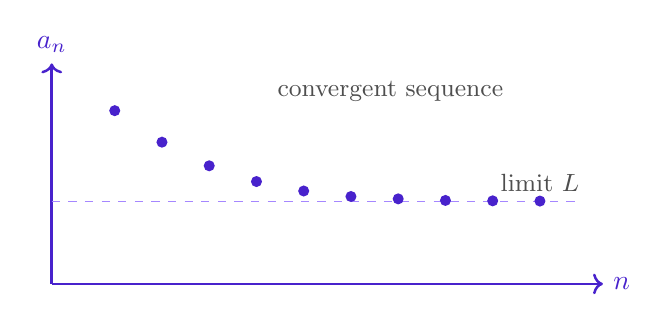
\begin{tikzpicture}[scale=1]
\draw[novelPurpleDark, line width=0.9pt, ->] (0,0) -- (7,0) node[right] {$n$};
\draw[novelPurpleDark, line width=0.9pt, ->] (0,0) -- (0,2.8) node[above] {$a_n$};
\draw[novelPurpleLine, dashed] (0,1.05) -- (6.7,1.05);
\node[text=npgray] at (6.2,1.28) {\small limit \(L\)};

\foreach \x/\y in {0.8/2.2,1.4/1.8,2.0/1.5,2.6/1.30,3.2/1.18,3.8/1.11,4.4/1.08,5.0/1.06,5.6/1.055,6.2/1.052}
{
    \fill[novelPurpleDark] (\x,\y) circle (2pt);
}
\node[text=npgray] at (4.3,2.45) {\small convergent sequence};
\end{tikzpicture}
\end{center}
}

\newcommand{\seqdivergeoscfigure}{
\begin{center}
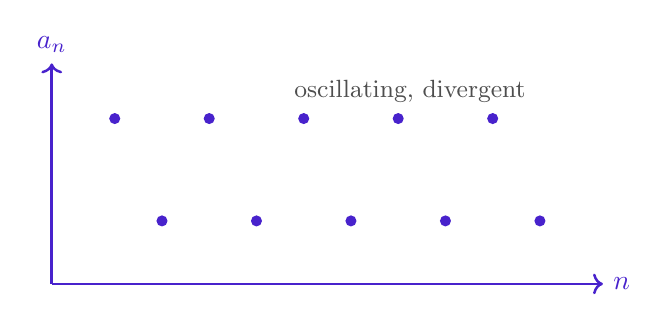
\begin{tikzpicture}[scale=1]
\draw[novelPurpleDark, line width=0.9pt, ->] (0,0) -- (7,0) node[right] {$n$};
\draw[novelPurpleDark, line width=0.9pt, ->] (0,0) -- (0,2.8) node[above] {$a_n$};

\foreach \x/\y in {0.8/2.1,1.4/0.8,2.0/2.1,2.6/0.8,3.2/2.1,3.8/0.8,4.4/2.1,5.0/0.8,5.6/2.1,6.2/0.8}
{
    \fill[novelPurpleDark] (\x,\y) circle (2pt);
}
\node[text=npgray] at (4.55,2.45) {\small oscillating, divergent};
\end{tikzpicture}
\end{center}
}

\newcommand{\seqdivergetoinftyfigure}{
\begin{center}
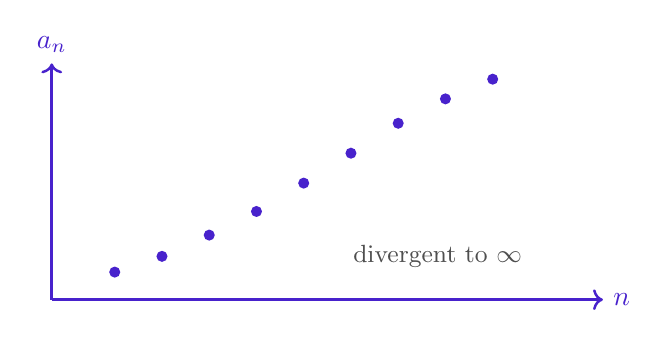
\begin{tikzpicture}[scale=1]
\draw[novelPurpleDark, line width=0.9pt, ->] (0,0) -- (7,0) node[right] {$n$};
\draw[novelPurpleDark, line width=0.9pt, ->] (0,0) -- (0,3.0) node[above] {$a_n$};

\foreach \x/\y in {0.8/0.35,1.4/0.55,2.0/0.82,2.6/1.12,3.2/1.48,3.8/1.86,4.4/2.24,5.0/2.55,5.6/2.8}
{
    \fill[novelPurpleDark] (\x,\y) circle (2pt);
}
\node[text=npgray] at (4.9,0.55) {\small divergent to \(\infty\)};
\end{tikzpicture}
\end{center}
}

\newcommand{\seriespartialsumfigure}{
\begin{center}
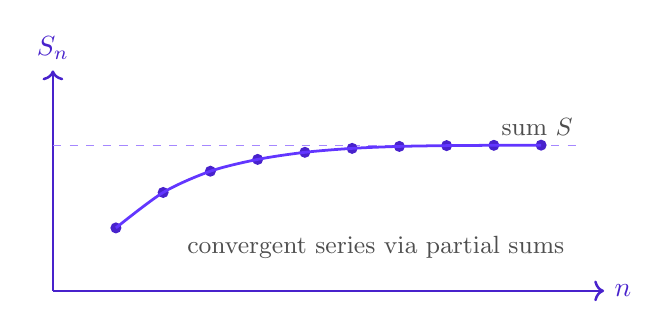
\begin{tikzpicture}[scale=1]
\draw[novelPurpleDark, line width=0.9pt, ->] (0,0) -- (7,0) node[right] {$n$};
\draw[novelPurpleDark, line width=0.9pt, ->] (0,0) -- (0,2.8) node[above] {$S_n$};
\draw[novelPurpleLine, dashed] (0,1.85) -- (6.7,1.85);
\node[text=npgray] at (6.15,2.08) {\small sum \(S\)};

\foreach \x/\y in {0.8/0.8,1.4/1.25,2.0/1.52,2.6/1.67,3.2/1.76,3.8/1.81,4.4/1.835,5.0/1.845,5.6/1.849,6.2/1.851}
{
    \fill[novelPurpleDark] (\x,\y) circle (2pt);
}
\draw[novelPurple, line width=1pt, smooth] plot coordinates {(0.8,0.8) (1.4,1.25) (2.0,1.52) (2.6,1.67) (3.2,1.76) (3.8,1.81) (4.4,1.835) (5.0,1.845) (5.6,1.849) (6.2,1.851)};
\node[text=npgray] at (4.1,0.55) {\small convergent series via partial sums};
\end{tikzpicture}
\end{center}
}

\newcommand{\geomconvergencefigure}{
\begin{center}
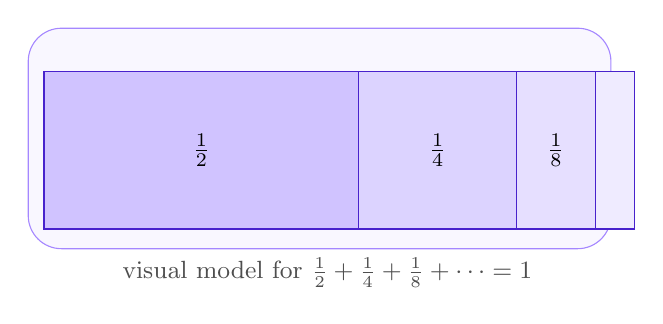
\begin{tikzpicture}[scale=1]
\fill[softlav, rounded corners=12pt] (-0.2,-0.25) rectangle (7.2,2.55);
\draw[novelPurpleLine, rounded corners=12pt] (-0.2,-0.25) rectangle (7.2,2.55);

\draw[fill=novelPurple!30, draw=novelPurpleDark] (0,0) rectangle (4,2);
\draw[fill=novelPurple!22, draw=novelPurpleDark] (4,0) rectangle (6,2);
\draw[fill=novelPurple!16, draw=novelPurpleDark] (6,0) rectangle (7,2);
\draw[fill=novelPurple!10, draw=novelPurpleDark] (7,0) rectangle (7.5,2);

\node at (2,1) {\(\frac12\)};
\node at (5,1) {\(\frac14\)};
\node at (6.5,1) {\(\frac18\)};
\node[text=npgray] at (3.6,-0.55) {\small visual model for \( \frac12+\frac14+\frac18+\cdots = 1 \)};
\end{tikzpicture}
\end{center}
}

% =========================================================
% COVER PAGE
% =========================================================
\begin{titlepage}
\centering
\vspace*{2.0cm}

{\fontsize{28}{32}\selectfont\bfseries\color{novelPurpleDark} AP Calculus BC\par}
\vspace{0.4cm}
{\fontsize{28}{32}\selectfont\bfseries\color{novelPurpleDark} Unit 10: Infinite Sequences and Series\par}

\vspace{0.8cm}
{\Large\color{novelPurple} Revised Novel Prep Edition\par}

\vspace{1.0cm}

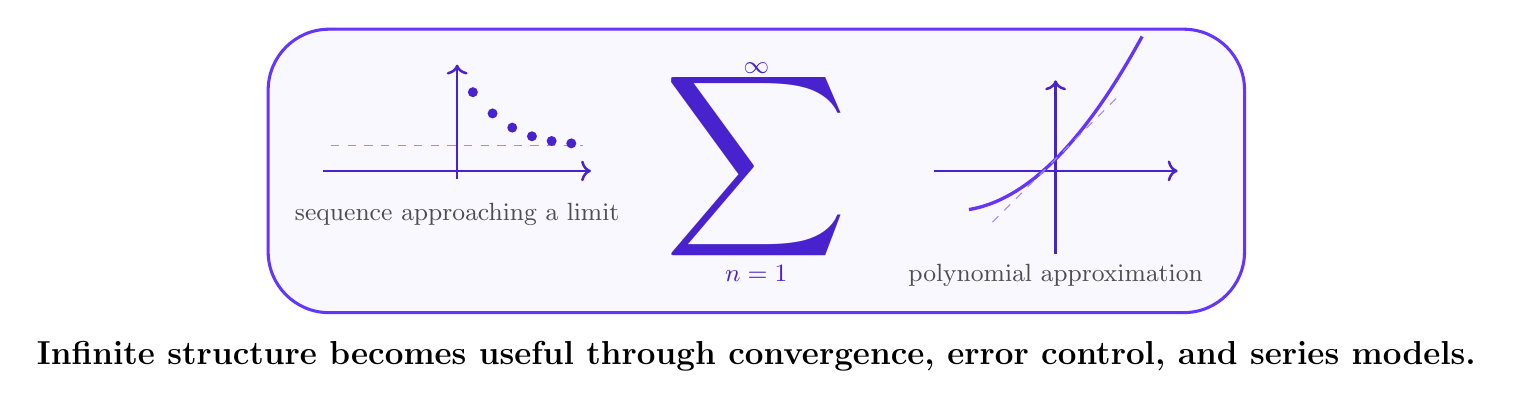
\begin{tikzpicture}[scale=1]
\fill[softlav,rounded corners=22pt] (-6.2,-1.8) rectangle (6.2,1.8);
\draw[novelPurple, line width=1.1pt, rounded corners=22pt] (-6.2,-1.8) rectangle (6.2,1.8);

% left sequence plot
\begin{scope}[shift={(-3.8,0)}]
\draw[novelPurpleDark, line width=0.9pt, ->] (-1.7,0) -- (1.7,0);
\draw[novelPurpleDark, line width=0.9pt, ->] (0,-0.1) -- (0,1.35);
\draw[novelPurpleLine, dashed] (-1.6,0.32) -- (1.6,0.32);
\foreach \x/\y in {0.2/1.0,0.45/0.73,0.7/0.55,0.95/0.44,1.2/0.38,1.45/0.35} {
  \fill[novelPurpleDark] (\x,\y) circle (1.8pt);
}
\node[text=npgray] at (0,-0.55) {\small sequence approaching a limit};
\end{scope}

% sigma
\node[novelPurpleDark] at (0,0.05) {\fontsize{46}{46}\selectfont $\displaystyle \sum$};
\node[novelPurpleDark] at (0,-1.3) {\small $n=1$};
\node[novelPurpleDark] at (0,1.3) {\small $\infty$};

% right polynomial approximation
\begin{scope}[shift={(3.8,0)}]
\draw[novelPurpleDark, line width=0.9pt, ->] (-1.55,0) -- (1.55,0);
\draw[novelPurpleDark, line width=0.9pt, ->] (0,-1.05) -- (0,1.15);
\draw[novelPurple, line width=1.2pt, smooth, domain=-1.1:1.1, samples=120]
plot (\x,{0.15 + \x + 0.38*\x*\x});
\draw[novelPurpleLine, dashed, smooth, domain=-0.8:0.8, samples=100]
plot (\x,{0.15 + \x});
\node[text=npgray] at (0,-1.32) {\small  polynomial approximation};
\end{scope}

\node[align=center] at (0,-2.35) {\large\bfseries Infinite structure becomes useful through convergence, error control, and series models.};
\end{tikzpicture}

\vfill

\begin{minipage}{0.84\textwidth}
\begin{notebox}{Design Goals for This Revision}
\begin{itemize}
    \item Keep the overall chapter sequence and mathematical scope of your original Unit 10.
    \item Upgrade the visual style to match the optimized Novel Prep Unit 1 system.
    \item Clarify the logic behind convergence tests instead of presenting them as disconnected rules.
    \item Strengthen the transition from convergence questions to Taylor and power series ideas.
    \item Build a polished chapter useful for both first instruction and AP BC review.
\end{itemize}
\end{notebox}
\end{minipage}

\vfill

{\large\textbf{Novel Prep Learning Center}}\\[0.25em]
{\large J. Z}

\end{titlepage}

\tableofcontents
\newpage

% =========================================================
% Force chapter numbering to start at 10
% =========================================================
\setcounter{section}{9}
\section{Infinite Sequences and Series}

\begin{theorybox}{Big Idea}
A finite process ends, so it can be computed directly.  
An infinite process must be understood through limits.

This unit asks:
\begin{center}
\itshape
When does an infinite expression settle down, when does it fail, and how can infinite series represent functions?
\end{center}
\end{theorybox}

\begin{notebox}{Teaching Philosophy for This Unit}
Students should not memorize a list of tests without understanding the structure behind them.
The real flow of Unit 10 is:
\[
\text{sequence} \to \text{series} \to \text{convergence tests} \to \text{error bounds} \to \text{power series} \to \text{Taylor models}.
\]
The chapter becomes much easier once students understand that every test answers a specific type of question.
\end{notebox}

\begin{theorybox}{Core Idea}
A sequence studies individual terms \(a_n\).  
A series studies accumulated sums
\[
S_n=a_1+a_2+\cdots+a_n.
\]
Series convergence is always about the behavior of the partial sums \(\{S_n\}\).
\end{theorybox}

\apcheckpoint{
Always distinguish between:
\begin{itemize}
    \item the sequence \(\{a_n\}\), and
    \item the series \(\sum a_n\).
\end{itemize}
The terms of a sequence may go to \(0\), but that alone does not guarantee the series converges.
}

\begin{theorybox}{Unit Overview}
This revised unit is organized around the following ideas:
\begin{enumerate}
    \item defining and analyzing sequences
    \item interpreting infinite series through partial sums
    \item choosing convergence or divergence tests appropriately
    \item estimating approximation error
    \item moving from convergence questions to power series and Taylor series
    \item using polynomial approximations to represent more complicated functions locally
\end{enumerate}
\end{theorybox}

\begin{theorybox}{AP Unit 10 Topic Map}
\renewcommand{\arraystretch}{1.25}
\begin{tabularx}{\textwidth}{@{}p{0.20\textwidth}p{0.30\textwidth}X@{}}
\toprule
Topic & Focus & Main Skill Emphasis \\
\midrule
10.1 Sequences and Infinite Series & terms, limits, partial sums & distinguish term behavior from sum behavior \\
10.2 Geometric Series & exact infinite sums & identify ratio and convergence quickly \\
10.3 \(n\)th-Term Test & necessary divergence test & reject impossible convergence \\
10.4 Integral Test & continuous comparison model & connect integrals to series \\
10.5 Harmonic and \(p\)-Series & standard benchmark families & classify basic models fast \\
10.6 Comparison Tests & relative size and asymptotics & compare to known benchmark series \\
10.7 Alternating Series & sign-changing convergence & verify monotone decrease to zero \\
10.8 Ratio Test & factorial/exponential behavior & handle growth efficiently \\
10.9 Absolute or Conditional Convergence & convergence type & classify more precisely \\
10.10 Alternating Series Error Bound & approximation accuracy & choose \(n\) for a target error \\
10.11 Taylor Polynomial Approximations & local finite models & build low-degree approximations \\
10.12 Lagrange Error Bound & accuracy of approximation & bound remainder size \\
10.13 Radius and Interval of Convergence & where a power series works & test endpoints carefully \\
10.14 Taylor / Maclaurin Series & infinite polynomial representation & derive standard series \\
10.15 Representing Functions as Power Series & operations on known series & create new series efficiently \\
\bottomrule
\end{tabularx}
\end{theorybox}

% =========================================================
\unitchapter{Defining Convergent and Divergent Infinite Series}

\unitsubtopic{Sequence}

\begin{theorybox}{Definition of a Sequence}
A \textbf{sequence} is a function whose domain is the positive integers.
Instead of standard function notation, we usually write
\[
\{a_n\}_{n=1}^{\infty}
\quad \text{or simply} \quad
\{a_n\}.
\]
\end{theorybox}

\begin{center}
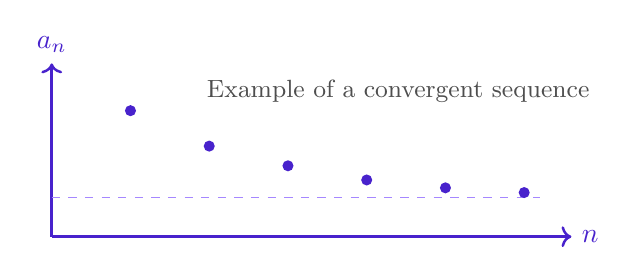
\begin{tikzpicture}[scale=1.0]
\draw[novelPurpleDark, line width=0.9pt, ->] (0,0) -- (6.6,0) node[right] {$n$};
\draw[novelPurpleDark, line width=0.9pt, ->] (0,0) -- (0,2.2) node[above] {$a_n$};
\draw[novelPurpleLine, dashed] (0,0.5) -- (6.2,0.5);
\foreach \x/\y in {1/1.6,2/1.15,3/0.9,4/0.72,5/0.62,6/0.56}
{
\fill[novelPurpleDark] (\x,\y) circle (2pt);
}
\node[text=npgray] at (4.4,1.85) {\small Example of a convergent sequence};
\end{tikzpicture}
\end{center}

\example{Listing the terms of a sequence}
List the first four terms of each sequence:
\[
a_n=3+(-1)^n,\qquad
b_n=\frac{n}{1-2n},\qquad
c_n=\frac{n^2}{2n-1}.
\]

\solution
For \(a_n\),
\[
a_1=2,\quad a_2=4,\quad a_3=2,\quad a_4=4.
\]

For \(b_n\),
\[
b_1=-1,\quad b_2=-\frac23,\quad b_3=-\frac35,\quad b_4=-\frac47.
\]

For \(c_n\),
\[
c_1=1,\quad c_2=\frac43,\quad c_3=\frac97,\quad c_4=\frac{16}{15}.
\]

\example{A recursively defined sequence}
Suppose \(d_1=25\) and
\[
d_{n+1}=d_n-5.
\]
List the first four terms.

\solution
\[
d_1=25,\quad d_2=20,\quad d_3=15,\quad d_4=10.
\]

\unitsubtopic{Limit of a Sequence}

\begin{theorybox}{Definition of the Limit of a Sequence}
We say
\[
\lim_{n\to\infty} a_n = L
\]
if the terms of the sequence get arbitrarily close to \(L\) as \(n\) becomes arbitrarily large.

If the limit exists, the sequence \textbf{converges}.  
If the limit does not exist, the sequence \textbf{diverges}.

\end{theorybox}

\seqconvergefigure
\seqdivergeoscfigure
\seqdivergetoinftyfigure


\begin{theorybox}{Sequence-Function Connection}
If \(f(n)=a_n\) for positive integers \(n\), and
\[
\lim_{x\to\infty}f(x)=L,
\]
then
\[
\lim_{n\to\infty}a_n=L.
\]
This lets us evaluate many sequence limits using ordinary limit techniques.
\end{theorybox}

\example{Finding the limit of a sequence}
Find
\[
\lim_{n\to\infty}\left(1+\frac1n\right)^n.
\]

\solution
Using the standard limit,
\[
\lim_{x\to\infty}\left(1+\frac1x\right)^x=e.
\]
Therefore,
\[
\lim_{n\to\infty}\left(1+\frac1n\right)^n=e.
\]

\example{Determining convergence or divergence}
Determine whether each sequence converges or diverges:
\[
a_n=3+(-1)^n,\qquad
b_n=\frac{n}{1-2n}.
\]

\solution
The sequence \(a_n\) alternates between \(2\) and \(4\), so it does not approach one value and diverges.

For \(b_n\),
\[
\frac{n}{1-2n}=\frac{1}{\frac1n-2}.
\]
As \(n\to\infty\), \(\frac1n\to 0\), so
\[
\lim_{n\to\infty}\frac{n}{1-2n}=-\frac12.
\]
Thus \(\{b_n\}\) converges to \(-\frac12\).

\begin{theorybox}{Properties of Limits of Sequences}
If \(\lim_{n\to\infty}a_n=L\) and \(\lim_{n\to\infty}b_n=K\), then:
\begin{enumerate}
    \item \(\lim(a_n\pm b_n)=L\pm K\)
    \item \(\lim(ca_n)=cL\)
    \item \(\lim(a_nb_n)=LK\)
    \item \(\lim\dfrac{a_n}{b_n}=\dfrac{L}{K}\), provided \(K\neq 0\)
\end{enumerate}
\end{theorybox}

\begin{theorybox}{Absolute Value Theorem}
If
\[
\lim_{n\to\infty}|a_n|=0,
\]
then
\[
\lim_{n\to\infty}a_n=0.
\]
\end{theorybox}

\example{Applying the absolute value theorem}
Determine the limit of
\[
a_n=\frac{(-1)^n}{n}.
\]

\solution
\[
|a_n|=\frac1n\to 0.
\]
Therefore
\[
\lim_{n\to\infty}\frac{(-1)^n}{n}=0.
\]
\newpage
\unitsubtopic{Monotonic Sequences and Bounded Sequences}

\begin{theorybox}{Monotonic Sequence}
A sequence is \textbf{monotonic increasing} if
\[
a_1\le a_2\le a_3\le \cdots
\]
and \textbf{monotonic decreasing} if
\[
a_1\ge a_2\ge a_3\ge \cdots.
\]
\end{theorybox}

\begin{theorybox}{Bounded Sequence}
A sequence is:
\begin{itemize}
    \item \textbf{bounded above} if \(a_n\le M\) for all \(n\),
    \item \textbf{bounded below} if \(N\le a_n\) for all \(n\),
    \item \textbf{bounded} if it is both bounded above and bounded below.
\end{itemize}
\end{theorybox}

\begin{theorybox}{Bounded Monotonic Sequence Theorem}
If a sequence is bounded and monotonic, then it converges.
\end{theorybox}

\begin{center}
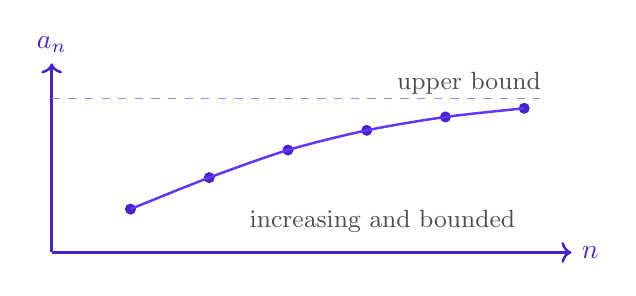
\begin{tikzpicture}[scale=1.0]
\draw[novelPurpleDark, line width=0.9pt, ->] (0,0) -- (6.6,0) node[right] {$n$};
\draw[novelPurpleDark, line width=0.9pt, ->] (0,0) -- (0,2.4) node[above] {$a_n$};
\draw[novelPurpleLine, dashed] (0,1.95) -- (6.2,1.95);
\node[text=npgray] at (5.3,2.15) {\small upper bound};
\foreach \x/\y in {1/0.55,2/0.95,3/1.3,4/1.55,5/1.72,6/1.83}
{
\fill[novelPurpleDark] (\x,\y) circle (2pt);
}
\draw[novelPurple, line width=0.9pt, smooth] plot coordinates {(1,0.55) (2,0.95) (3,1.3) (4,1.55) (5,1.72) (6,1.83)};
\node[text=npgray] at (4.2,0.4) {\small increasing and bounded};
\end{tikzpicture}
\end{center}

\example{Determining whether a sequence is monotonic}
Determine whether the following are monotonic:
\[
a_n=3+(-1)^n,\qquad
b_n=\frac{2n}{n+1},\qquad
c_n=\frac{n^2}{2n-1}.
\]

\solution
\begin{itemize}
    \item \(a_n\) alternates, so it is not monotonic.
    \item \(b_n=\frac{2n}{n+1}\) is increasing.
    \item \(c_n=\frac{n^2}{2n-1}\) is not monotonic from the beginning.
\end{itemize}

\example{Using the bounded monotonic sequence theorem}
Discuss the following:
\[
a_n=\frac1n,\qquad
b_n=\frac{n^2}{n+1},\qquad
c_n=(-1)^n.
\]

\solution
\begin{itemize}
    \item \(\frac1n\) is decreasing and bounded below by \(0\), so it converges.
    \item \(\frac{n^2}{n+1}\) is unbounded, so it diverges.
    \item \((-1)^n\) is bounded but not monotonic, and it diverges.
\end{itemize}
\newpage
\unitsubtopic{Infinite Series}

\begin{theorybox}{Infinite Series}
An \textbf{infinite series} is the sum of the terms of an infinite sequence:
\[
\sum_{n=1}^{\infty} a_n = a_1+a_2+a_3+\cdots.
\]
\end{theorybox}


A series does \emph{not} converge because its terms look small.  
A series converges only if its partial sums settle to a finite number.

\seriespartialsumfigure


\begin{theorybox}{Partial Sums and Series Convergence}
Define the \(n\)th partial sum by
\[
S_n=a_1+a_2+\cdots+a_n.
\]
If the sequence \(\{S_n\}\) converges to \(S\), then
\[
\sum_{n=1}^{\infty} a_n=S.
\]
If \(\{S_n\}\) diverges, then the series diverges.
\end{theorybox}

\begin{theorybox}{Telescoping Series}
A \textbf{telescoping series} is a series in which many terms cancel when the partial sums are expanded.
\end{theorybox}

\begin{center}
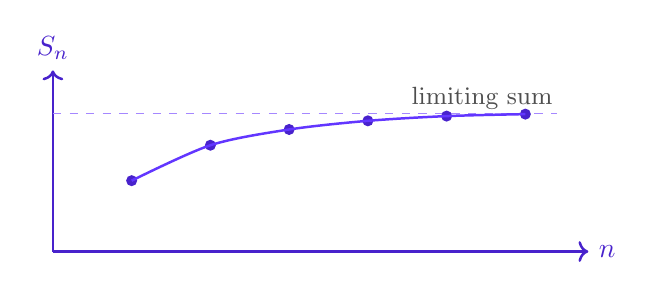
\begin{tikzpicture}[scale=1.0]
\draw[novelPurpleDark, line width=0.9pt, ->] (0,0) -- (6.8,0) node[right] {$n$};
\draw[novelPurpleDark, line width=0.9pt, ->] (0,0) -- (0,2.3) node[above] {$S_n$};
\draw[novelPurpleLine, dashed] (0,1.75) -- (6.4,1.75);
\foreach \x/\y in {1/0.9,2/1.35,3/1.55,4/1.66,5/1.72,6/1.745}
{
\fill[novelPurpleDark] (\x,\y) circle (2pt);
}
\draw[novelPurple, line width=0.9pt, smooth] plot coordinates {(1,0.9) (2,1.35) (3,1.55) (4,1.66) (5,1.72) (6,1.745)};
\node[text=npgray] at (5.45,1.95) {\small limiting sum};
\end{tikzpicture}
\end{center}

\example{Convergent and divergent series}
Determine whether each series converges or diverges:
\[
\sum_{n=1}^{\infty}\frac1{2^n},
\qquad
\sum_{n=1}^{\infty}\left(\frac1n-\frac1{n+1}\right),
\qquad
\sum_{n=1}^{\infty}1.
\]

\solution
The first is geometric and converges to \(1\).

The second telescopes:
\[
S_n=1-\frac1{n+1}\to 1,
\]
so it converges to \(1\).

The third has partial sums \(S_n=n\to\infty\), so it diverges.

\example{Reading convergence through partial sums}
Explain why a series can converge even though it has infinitely many terms.

\solution
A series converges when the \emph{partial sums} approach a finite number. The number of terms is infinite, but the accumulated total can still stabilize.

% =========================================================
\unitchapter{Geometric Series}

\begin{theorybox}{Geometric Series}
A geometric series has the form
\[
\sum_{n=0}^{\infty} ar^n=a+ar+ar^2+\cdots,
\]
where \(a\neq 0\) and \(r\) is the common ratio.
\end{theorybox}

\begin{theorybox}{Convergent and Divergent Geometric Series}
A geometric series:
\[
\sum_{n=0}^{\infty} ar^n
\]
\begin{itemize}
    \item diverges if \(|r|\ge 1\),
    \item converges if \(|r|<1\), and then
    \[
    \sum_{n=0}^{\infty} ar^n=\frac{a}{1-r}.
    \]
\end{itemize}
\end{theorybox}

One of the best ways to understand a convergent geometric series is through area.

\geomconvergencefigure


\example{Convergent and divergent geometric series}
Determine whether each converges:
\[
\sum_{n=0}^{\infty}\frac{3}{2^n},
\qquad
\sum_{n=0}^{\infty}\left(\frac32\right)^n.
\]

\solution
The first has \(a=3\), \(r=\frac12\), so it converges to
\[
\frac{3}{1-\frac12}=6.
\]
The second has \(|r|=\frac32>1\), so it diverges.

\example{Geometric series for a repeating decimal}
Write \(0.\overline{08}\) as a ratio of two integers.

\solution
\[
0.\overline{08}
=
\frac{8}{100}+\frac{8}{100^2}+\frac{8}{100^3}+\cdots
\]
This is geometric with
\[
a=\frac{8}{100},\qquad r=\frac{1}{100}.
\]
Thus
\[
0.\overline{08}
=
\frac{\frac{8}{100}}{1-\frac{1}{100}}
=
\frac{8}{99}.
\]

\apcheckpoint{
For a geometric series, the entire decision comes from the ratio \(r\).
}

% =========================================================
\unitchapter{The \texorpdfstring{$n$}{n}th Term Test for Divergence}

\begin{theorybox}{Limit of the \(n\)th Term of a Convergent Series}
If
\[
\sum_{n=1}^{\infty}a_n
\]
converges, then
\[
\lim_{n\to\infty}a_n=0.
\]
\end{theorybox}

\begin{theorybox}{\(n\)th-Term Test for Divergence}
If
\[
\lim_{n\to\infty}a_n\neq 0
\]
or the limit does not exist, then
\[
\sum_{n=1}^{\infty}a_n
\]
diverges.
\end{theorybox}

\example{Using the \(n\)th-term test}
Determine whether the following series diverge:
\[
\sum_{n=0}^{\infty}2^n,\qquad
\sum_{n=1}^{\infty}\frac{n!}{2n!+1},\qquad
\sum_{n=1}^{\infty}\frac1n.
\]

\solution
For \(\sum 2^n\), the term limit is \(\infty\), so the series diverges.

For \(\sum \frac{n!}{2n!+1}\), the term limit is \(\frac12\), so it diverges.

For \(\sum \frac1n\), the term limit is \(0\), so the test is inconclusive.

\example{A nonzero term limit}
Determine whether
\[
\sum_{n=1}^{\infty}\frac{3n+2}{3n+5}
\]
converges.

\solution
\[
\lim_{n\to\infty}\frac{3n+2}{3n+5}=1\neq 0.
\]
Therefore the series diverges.

% =========================================================
\unitchapter{Integral Test for Convergence}

\begin{theorybox}{Integral Test}
If \(f\) is continuous, positive, and decreasing for \(x\ge N\), and \(a_n=f(n)\), then
\[
\sum_{n=N}^{\infty} a_n
\]
and
\[
\int_N^{\infty}f(x)\,dx
\]
either both converge or both diverge.
\end{theorybox}

\example{Applying the Integral Test}
Apply the Integral Test to
\[
\sum_{n=1}^{\infty}\frac{1}{n^2+1}.
\]

\solution
Let
\[
f(x)=\frac{1}{x^2+1}.
\]
This function is continuous, positive, and decreasing for \(x\ge 1\).

Now compute:
\[
\int_1^\infty \frac{1}{x^2+1}\,dx
=
\lim_{b\to\infty}[\arctan x]_1^b
=
\frac{\pi}{2}-\frac{\pi}{4}
=
\frac{\pi}{4}.
\]
So the integral converges, and therefore the series converges.

\example{A divergent logarithmic example}
Determine whether
\[
\sum_{n=2}^{\infty}\frac{1}{n\ln n}
\]
converges.

\solution
Let
\[
f(x)=\frac{1}{x\ln x}.
\]
Then
\[
\int_2^\infty \frac{1}{x\ln x}\,dx
=
\int_{\ln 2}^{\infty}\frac{1}{u}\,du
\]
with \(u=\ln x\), which diverges. Therefore the series diverges.

% =========================================================
\unitchapter{Harmonic Series and \texorpdfstring{$p$}{p}-Series}
\unitsubtopic{\texorpdfstring{$p$}{p}-Series- Test}

\begin{theorybox}{\(p\)-Series}
A series of the form
\[
\sum_{n=1}^{\infty}\frac{1}{n^p}
\]
is called a \textbf{\(p\)-series}.
\end{theorybox}

\begin{theorybox}{The Harmonic Series}
The series
\[
\sum_{n=1}^{\infty}\frac{1}{n}
\]
is called the \textbf{harmonic series}, and it \textbf{diverges}.
\end{theorybox}

\example{Why does the harmonic series diverge?}
At first glance, the terms \(\frac{1}{n}\) get smaller and smaller, so it may seem that the series should converge.

However, this is \textbf{not enough} to guarantee convergence.

\solution
We group the terms as follows:
\[
\left(1\right)
+
\left(\frac{1}{2}\right)
+
\left(\frac{1}{3}+\frac{1}{4}\right)
+
\left(\frac{1}{5}+\cdots+\frac{1}{8}\right)
+
\left(\frac{1}{9}+\cdots+\frac{1}{16}\right)
+\cdots
\]

Now estimate each group from below:

\[
\frac{1}{3}+\frac{1}{4} > \frac{1}{4}+\frac{1}{4} = \frac{1}{2}
\]

\[
\frac{1}{5}+\cdots+\frac{1}{8} > 4\cdot \frac{1}{8} = \frac{1}{2}
\]

\[
\frac{1}{9}+\cdots+\frac{1}{16} > 8\cdot \frac{1}{16} = \frac{1}{2}
\]

Each group is at least \(\frac{1}{2}\), so the partial sums grow like
\[
1 + \frac{1}{2} + \frac{1}{2} + \frac{1}{2} + \cdots \to \infty.
\]

Therefore, the harmonic series diverges.

\bigskip

\textbf{Key takeaway:}  
Even though \(\frac{1}{n} \to 0\), the terms do not decrease fast enough, so the series diverges.
\end{solution}
\newpage
\example{\(p\)-series practice}
Determine whether each series converges or diverges:
\[
\sum_{n=1}^{\infty}\frac{1}{n^5},
\qquad
\sum_{n=1}^{\infty}\frac{1}{n^{4/5}},
\qquad
\sum_{n=1}^{\infty}\frac{1}{n}.
\]

\solution
These are all \(p\)-series of the form
\[
\sum_{n=1}^{\infty}\frac{1}{n^p}.
\]

\[
p=5>1 \Rightarrow \text{convergent}
\]

\[
p=\frac45<1 \Rightarrow \text{divergent}
\]

\[
p=1 \Rightarrow \text{harmonic series} \Rightarrow \text{divergent}
\]

So the answers are:
\[
\sum_{n=1}^{\infty}\frac{1}{n^5}\text{ converges},\qquad
\sum_{n=1}^{\infty}\frac{1}{n^{4/5}}\text{ diverges},\qquad
\sum_{n=1}^{\infty}\frac{1}{n}\text{ diverges}.
\]
\end{solution}

\example{Rewriting into \(p\)-series form}
Determine whether each series converges or diverges:
\[
\sum_{n=1}^{\infty}\frac{1}{\sqrt[3]{n}},
\qquad
\sum_{n=1}^{\infty}\frac{1}{n\sqrt n},
\qquad
\sum_{n=1}^{\infty}\frac{1}{\sqrt[4]{n^5}}.
\]

\solution


\bigskip


\[
\sum_{n=1}^{\infty}\frac{1}{\sqrt[3]{n}}\text{ diverges},\qquad
\sum_{n=1}^{\infty}\frac{1}{n\sqrt n}\text{ converges},\qquad
\sum_{n=1}^{\infty}\frac{1}{\sqrt[4]{n^5}}\text{ converges}.
\]
\end{solution}
\newpage
\example{Harder \(p\)-series practice}
Determine whether each series converges or diverges:
\[
\sum_{n=1}^{\infty}\frac{1}{n^{2/3}+5},
\qquad
\sum_{n=1}^{\infty}\frac{n^2+1}{n^5},
\qquad
\sum_{n=1}^{\infty}\frac{\sqrt{n}+3}{n^2-1}.
\]

\solution
These are not written exactly as \(p\)-series, so we look at the dominant terms for large \(n\).

\bigskip

For
\[
\sum_{n=1}^{\infty}\frac{1}{n^{2/3}+5},
\]
the dominant term in the denominator is \(n^{2/3}\), so
\[
\frac{1}{n^{2/3}+5}\sim \frac{1}{n^{2/3}}.
\]
This behaves like a \(p\)-series with
\[
p=\frac23<1,
\]
so the series diverges.

\bigskip

For
\[
\sum_{n=1}^{\infty}\frac{n^2+1}{n^5},
\]
the dominant term in the numerator is \(n^2\), so
\[
\frac{n^2+1}{n^5}\sim \frac{n^2}{n^5}=\frac{1}{n^3}.
\]
This behaves like a \(p\)-series with
\[
p=3>1,
\]
so the series converges.

\bigskip

For
\[
\sum_{n=1}^{\infty}\frac{\sqrt{n}+3}{n^2-1},
\]
the dominant term in the numerator is \(\sqrt n\), and the dominant term in the denominator is \(n^2\), so
\[
\frac{\sqrt n+3}{n^2-1}\sim \frac{\sqrt n}{n^2}=\frac{1}{n^{3/2}}.
\]
This behaves like a \(p\)-series with
\[
p=\frac32>1,
\]
so the series converges.

\bigskip

Therefore,
\[
\sum_{n=1}^{\infty}\frac{1}{n^{2/3}+5}\text{ diverges},\qquad
\sum_{n=1}^{\infty}\frac{n^2+1}{n^5}\text{ converges},\qquad
\sum_{n=1}^{\infty}\frac{\sqrt{n}+3}{n^2-1}\text{ converges}.
\]

\bigskip

\textbf{Key idea:}  
For harder problems, first identify the dominant terms, then compare the series to a familiar \(p\)-series.
\end{solution}
\newpage
\unitsubtopic{Differences Between Geometric and P Series}
\begin{theorybox}{How to Tell the Difference Quickly}
When deciding whether a series is a \(p\)-series or a geometric series, first look at \textbf{where \(n\) appears}.

\bigskip

\[
\text{Is } n \text{ in the exponent?}
\]

\[
\begin{array}{c}
\Downarrow
\end{array}
\]

\[
\begin{array}{|c|}
\hline
\textbf{Yes} \\
\text{Then it is likely a geometric series.} \\
\text{Form: } \displaystyle \sum ar^n \\
\text{Check whether } |r|<1.\\
\hline
\end{array}
\qquad
\begin{array}{|c|}
\hline
\textbf{No} \\
\text{Then ask: does it look like } \displaystyle \sum \frac{1}{n^p}\textbf{?} \\
\text{If yes, it is a \(p\)-series.} \\
\text{Check whether } p>1.\\
\hline
\end{array}
\]

\bigskip

\textbf{Quick Reminder:}
\[
\frac{1}{n^2}
\quad\text{is a \(p\)-series}
\qquad\qquad
\left(\frac12\right)^n
\quad\text{is geometric}
\]

\bigskip

\textbf{Key idea:}
\[
n \text{ in the exponent } \Rightarrow \text{ geometric series}
\]
\[
n \text{ in the base or denominator power } \Rightarrow \text{ often a \(p\)-series}
\]
\end{theorybox}

\example{Classify the series}
For each series below, decide whether it is a \(p\)-series, a geometric series, or neither.

\[
\text{(a)}\ \sum_{n=1}^{\infty}\frac{1}{n^3}
\qquad
\text{(b)}\ \sum_{n=0}^{\infty}\left(\frac{2}{5}\right)^n
\qquad
\text{(c)}\ \sum_{n=1}^{\infty}\frac{3}{n^{1/2}}
\]
\[
\text{(d)}\ \sum_{n=1}^{\infty}\frac{1}{2^n}
\qquad
\text{(e)}\ \sum_{n=1}^{\infty}\frac{n+1}{n^2}
\qquad
\text{(f)}\ \sum_{n=1}^{\infty}\left(-3\right)^n
\]

\solution
\textbf{(a)} 
\[
\sum_{n=1}^{\infty}\frac{1}{n^3}
\]
This matches the form
\[
\sum \frac{1}{n^p}
\]
with \(p=3\), so it is a \textbf{\(p\)-series}.

\bigskip

\textbf{(b)}
\[
\sum_{n=0}^{\infty}\left(\frac{2}{5}\right)^n
\]
Here \(n\) is in the exponent, so this is a \textbf{geometric series} with
\[
r=\frac25.
\]

\bigskip

\textbf{(c)}
\[
\sum_{n=1}^{\infty}\frac{3}{n^{1/2}}
\]
The constant \(3\) does not matter. The main form is
\[
\sum \frac{1}{n^{1/2}},
\]
so this is a \textbf{\(p\)-series} with \(p=\frac12\).

\bigskip

\textbf{(d)}
\[
\sum_{n=1}^{\infty}\frac{1}{2^n}
=
\sum_{n=1}^{\infty}\left(\frac12\right)^n
\]
Since \(n\) is in the exponent, this is a \textbf{geometric series}.

\bigskip

\textbf{(e)}
\[
\sum_{n=1}^{\infty}\frac{n+1}{n^2}
\]
This is \textbf{not exactly} of the form
\[
\sum \frac{1}{n^p}
\]
and it is not geometric either, so it is \textbf{neither}.

\bigskip

\textbf{(f)}
\[
\sum_{n=1}^{\infty}(-3)^n
\]
Since \(n\) is in the exponent, this is a \textbf{geometric series} with
\[
r=-3.
\]

\bigskip

Therefore:
\[
\text{(a) \(p\)-series, \quad (b) geometric, \quad (c) \(p\)-series,}
\]
\[
\text{(d) geometric, \quad (e) neither, \quad (f) geometric.}
\]
\end{solution}

\example{Determine whether each series converges or diverges}
Classify each series first, then determine whether it converges or diverges.

\[
\text{(a)}\ \sum_{n=1}^{\infty}\frac{1}{n^{5/2}}
\qquad
\text{(b)}\ \sum_{n=0}^{\infty}\left(\frac{3}{4}\right)^n
\qquad
\text{(c)}\ \sum_{n=1}^{\infty}\frac{1}{n}
\]
\[
\text{(d)}\ \sum_{n=1}^{\infty}2^n
\qquad
\text{(e)}\ \sum_{n=1}^{\infty}\frac{1}{n^{2/3}}
\qquad
\text{(f)}\ \sum_{n=1}^{\infty}\left(-\frac12\right)^n
\]

\solution
\textbf{(a)}
\[
\sum_{n=1}^{\infty}\frac{1}{n^{5/2}}
\]
This is a \(p\)-series with
\[
p=\frac52>1,
\]
so it \textbf{converges}.

\bigskip

\textbf{(b)}
\[
\sum_{n=0}^{\infty}\left(\frac34\right)^n
\]
This is geometric with
\[
r=\frac34.
\]
Since
\[
|r|<1,
\]
it \textbf{converges}.

\bigskip

\textbf{(c)}
\[
\sum_{n=1}^{\infty}\frac{1}{n}
\]
This is a \(p\)-series with
\[
p=1,
\]
so it is the harmonic series and \textbf{diverges}.

\bigskip

\textbf{(d)}
\[
\sum_{n=1}^{\infty}2^n
\]
This is geometric with
\[
r=2.
\]
Since
\[
|r|>1,
\]
it \textbf{diverges}.

\bigskip

\textbf{(e)}
\[
\sum_{n=1}^{\infty}\frac{1}{n^{2/3}}
\]
This is a \(p\)-series with
\[
p=\frac23<1,
\]
so it \textbf{diverges}.

\bigskip

\textbf{(f)}
\[
\sum_{n=1}^{\infty}\left(-\frac12\right)^n
\]
This is geometric with
\[
r=-\frac12.
\]
Since
\[
|r|=\frac12<1,
\]
it \textbf{converges}.

\bigskip

Therefore:
\[
\text{(a) converges, \quad (b) converges, \quad (c) diverges,}
\]
\[
\text{(d) diverges, \quad (e) diverges, \quad (f) converges.}
\]
\end{solution}



% =========================================================
\unitchapter{Comparison Tests for Convergence}

\unitsubtopic{Comparison Tests for Convergence}

\begin{theorybox}{Direct Comparison Test}
Suppose \(0\le a_n\le b_n\) for all sufficiently large \(n\).
\begin{itemize}
    \item If \(\sum b_n\) converges, then \(\sum a_n\) converges.
    \item If \(\sum a_n\) diverges, then \(\sum b_n\) diverges.
\end{itemize}
\end{theorybox}

\noindent
{\color{novelPurple}\textbf{When to Think of Direct Comparison Test}}

\bigskip

Think of the Direct Comparison Test when you can \textbf{immediately compare} the terms with a known benchmark series using
\[
a_n \le b_n
\qquad\text{or}\qquad
a_n \ge b_n.
\]

\bigskip

\textbf{Use it when:}
\begin{itemize}
    \item the inequality is easy to see,
    \item the comparison is term by term,
    \item and the benchmark is a familiar convergent or divergent series.
\end{itemize}

\bigskip



\example{Direct comparison}
Determine whether
\[
\sum_{n=1}^{\infty}\frac{5}{2n^2+4n+3}
\]
converges or diverges.

\solution
Since
\[
0<\frac{5}{2n^2+4n+3}<\frac{5}{2n^2},
\]
and \(\sum \frac{5}{2n^2}\) converges, the given series converges.

\example{A divergent direct comparison}
Test
\[
\sum_{k=3}^{\infty}\frac{\ln k}{k}
\]
for convergence or divergence.

\solution
For \(k\ge 3\),
\[
\frac{\ln k}{k}>\frac{1}{k}.
\]
Since the harmonic series diverges, the given series diverges by direct comparison.
\newpage
\unitsubtopic{The Limit Comparison Test}

\begin{theorybox}{Limit Comparison Test}
Let \(a_n>0\) and \(b_n>0\). If
\[
\lim_{n\to\infty}\frac{a_n}{b_n}=L
\qquad\text{for some } 0<L<\infty,
\]
then \(a_n\) and \(b_n\) have the same long-term size.

Therefore,
\[
\sum_{n=1}^\infty a_n
\quad\text{and}\quad
\sum_{n=1}^\infty b_n
\]
either both converge or both diverge.

\medskip

\textbf{In other words:} if two positive sequences behave like constant multiples of each other for large \(n\), then their series have the same convergence behavior.
\end{theorybox}

\noindent
{\color{novelPurple}\textbf{How to Choose \(b_n\) Quickly}}



To apply the Limit Comparison Test, \(b_n\) should not be guessed randomly.  
Instead, choose \(b_n\) based on the \textbf{dominant behavior} of \(a_n\) as \(n \to \infty\).

\bigskip

\textbf{Core Idea:}  
Ignore constants and lower-order terms. Focus only on the terms that control the growth.

\bigskip

\textbf{Quick Steps:}
\begin{itemize}
    \item Ignore constants (like \(+3\), \(-5\))
    \item Keep highest power terms (dominant terms)
    \item Simplify the expression
    \item Match it to a known series (usually \( \frac{1}{n^p} \))
\end{itemize}

\bigskip

\textbf{Examples:}

\bigskip

\textbf{(1)}
\[
a_n = \frac{3n+5}{n^2+1}
\quad \Rightarrow \quad
\frac{3n}{n^2} = \frac{3}{n}
\]
\[
\Rightarrow \quad b_n = \frac{1}{n}
\]

\bigskip



\textbf{(2)}
\[
a_n = \frac{\sqrt{n}+2}{n^2+7}
\quad \Rightarrow \quad
\frac{\sqrt{n}}{n^2} = \frac{1}{n^{3/2}}
\]
\[
\Rightarrow \quad b_n = \frac{1}{n^{3/2}}
\]



\example{Limit comparison with a geometric series}
Test
\[
\sum_{n=1}^{\infty}\frac{1}{2^n-1}
\]
for convergence.

\solution
Let
\[
a_n=\frac{1}{2^n-1},\qquad b_n=\frac{1}{2^n}.
\]
Then
\[
\lim_{n\to\infty}\frac{a_n}{b_n}
=
\lim_{n\to\infty}\frac{2^n}{2^n-1}=1.
\]
Since \(\sum \frac1{2^n}\) converges, the given series also converges.

\example{Limit comparison with a \(p\)-series}
Determine whether
\[
\sum_{n=1}^{\infty}\frac{2n^2+3n}{\sqrt{5+n^5}}
\]
converges.

\solution
For large \(n\), the series behaves like
\[
\frac{2n^2}{n^{5/2}}=\frac{2}{\sqrt n}.
\]
So compare with
\[
b_n=\frac{1}{\sqrt n}.
\]
The limit comparison gives a positive finite constant, and because
\[
\sum \frac{1}{\sqrt n}
\]
diverges, the given series diverges.
\begin{theorybox}{Rule of thumb:}{}
    \begin{itemize}
    \item Easy inequality \(\rightarrow\) Direct Comparison Test
    \item Similar-looking expressions \(\rightarrow\) Limit Comparison Test
\end{itemize}

\end{theorybox}


% =========================================================
\unitchapter{Alternating Series}

\begin{theorybox}{Alternating Series}
A series with alternating signs is typically of the form
\[
\sum_{n=1}^{\infty}(-1)^{n-1}b_n
\quad\text{or}\quad
\sum_{n=1}^{\infty}(-1)^n b_n
\]
where \(b_n\ge 0\).
\end{theorybox}

\begin{theorybox}{Alternating Series Test}
If
\[
\sum_{n=1}^{\infty}(-1)^{n-1}b_n
\]
satisfies:
\begin{enumerate}
    \item \(b_n>0\),
    \item \(b_{n+1}\le b_n\),
    \item \(\lim_{n\to\infty}b_n=0\),
\end{enumerate}
then the series converges.
\end{theorybox}

\example{Applying the alternating series test}
Determine whether
\[
\sum_{n=1}^{\infty}\frac{(-1)^{n-1}}{n}
\]
converges.

\solution
Here \(b_n=\frac1n\), which is positive, decreasing, and tends to \(0\).  
So the series converges.

\example{A failing alternating series}
Determine whether
\[
\sum_{n=1}^{\infty}(-1)^{n-1}\frac{n}{n+1}
\]
converges.

\solution
The corresponding \(b_n=\frac{n}{n+1}\) does not approach \(0\), so the series diverges.

% =========================================================
\unitchapter{Ratio Test for Convergence}

\begin{theorybox}{Ratio Test}
For a series \(\sum a_n\), compute
\[
L=\lim_{n\to\infty}\left|\frac{a_{n+1}}{a_n}\right|.
\]
Then:
\begin{itemize}
    \item If \(L<1\), the series converges absolutely.
    \item If \(L>1\) or \(L=\infty\), the series diverges.
    \item If \(L=1\), the test is inconclusive.
\end{itemize}
\end{theorybox}

\example{Using the ratio test}
Determine whether
\[
\sum_{n=1}^{\infty}\frac{n}{2^n}
\]
converges.

\solution
Let
\[
a_n=\frac{n}{2^n}.
\]
Then
\[
\left|\frac{a_{n+1}}{a_n}\right|
=
\frac{n+1}{2n}\to \frac12<1.
\]
Therefore the series converges absolutely.

\example{A factorial-type series}
Determine whether
\[
\sum_{n=1}^{\infty}\frac{n^n}{n!}
\]
converges.

\solution
Let \(a_n=\frac{n^n}{n!}\). Then
\[
\frac{a_{n+1}}{a_n}
=
\frac{(n+1)^{n+1}}{(n+1)!}\cdot \frac{n!}{n^n}
=
\left(1+\frac1n\right)^n.
\]
Thus
\[
\lim_{n\to\infty}\frac{a_{n+1}}{a_n}=e>1.
\]
So the series diverges.

\example{A failure of the ratio test}
Determine the convergence or divergence of
\[
\sum_{n=1}^{\infty}(-1)^n\frac{\sqrt n}{n+1}.
\]

\solution
The absolute ratio limit simplifies to \(1\), so the Ratio Test is inconclusive.

% =========================================================
\unitchapter{Absolute or Conditional Convergence}

\begin{theorybox}{Absolute Convergence}
A series \(\sum a_n\) is \textbf{absolutely convergent} if
\[
\sum |a_n|
\]
converges.
\end{theorybox}

\begin{theorybox}{Conditional Convergence}
A series is \textbf{conditionally convergent} if
\[
\sum a_n
\]
converges but
\[
\sum |a_n|
\]
diverges.
\end{theorybox}

\begin{theorybox}{Absolute Convergence Theorem}
If
\[
\sum |a_n|
\]
converges, then
\[
\sum a_n
\]
also converges.
\end{theorybox}

\example{Absolute or conditional?}
Classify:
\[
\sum_{n=1}^{\infty}\frac{(-1)^n}{n^3},
\qquad
\sum_{n=1}^{\infty}\frac{(-1)^n}{\sqrt[3]{n}},
\qquad
\sum_{n=1}^{\infty}(-1)^n\frac{n}{2n+1}.
\]

\solution
\begin{itemize}
    \item \(\sum \frac{1}{n^3}\) converges, so the first is absolutely convergent.
    \item \(\sum \frac{1}{n^{1/3}}\) diverges, but the alternating version converges by AST, so the second is conditionally convergent.
    \item The term \(\frac{n}{2n+1}\not\to 0\), so the third diverges.
\end{itemize}

\example{A non-alternating absolute convergence example}
Determine whether
\[
\sum_{n=1}^{\infty}\frac{\sin n}{n^3}
\]
is convergent.

\solution
Since
\[
\left|\frac{\sin n}{n^3}\right|\le \frac{1}{n^3},
\]
and \(\sum \frac{1}{n^3}\) converges, the original series converges absolutely.

% =========================================================
\unitchapter{Alternating Series Error Bound}

\begin{theorybox}{Alternating Series Error Bound}
If
\[
S=\sum_{n=1}^{\infty}(-1)^{n-1}b_n
\]
is an alternating series satisfying the Alternating Series Test, and \(S_N\) is the \(N\)th partial sum, then
\[
|S-S_N|\le b_{N+1}.
\]
\end{theorybox}

\example{How many terms are needed?}
How many terms are needed to approximate
\[
\sum_{n=1}^{\infty}\frac{(-1)^{n-1}}{n}
\]
with error less than \(0.001\)?

\solution
We need
\[
\frac{1}{N+1}<0.001.
\]
So \(N+1>1000\), hence \(N=1000\) terms are enough.

\example{Approximating the sum of an alternating series}
Approximate
\[
\sum_{n=1}^{\infty}(-1)^{n+1}\frac{1}{n!}
\]
using the first six terms.

\solution
\[
S_6=1-\frac12+\frac16-\frac1{24}+\frac1{120}-\frac1{720}
=\frac{91}{144}\approx 0.63194.
\]
The next omitted term is
\[
\frac1{7!}=\frac1{5040}\approx 0.0002.
\]
So the true sum lies within \(0.0002\) of \(0.63194\).

% =========================================================
\unitchapter{Taylor Polynomial Approximations of Functions}
\unitsubtopic{Polynomial Approximations of Elementary Functions}

\begin{theorybox}{Polynomial Approximation}
A polynomial approximation of a function \(f(x)\) near \(x=a\) is a polynomial \(P_n(x)\) whose value and derivatives match those of \(f\) at \(x=a\).
\end{theorybox}

\begin{theorybox}{Taylor Polynomial}
The \(n\)th-degree Taylor polynomial of \(f\) centered at \(a\) is
\[
P_n(x)=f(a)+f'(a)(x-a)+\frac{f''(a)}{2!}(x-a)^2+\cdots+\frac{f^{(n)}(a)}{n!}(x-a)^n.
\]
\end{theorybox}

\example{First-degree approximation of \(e^x\)}
Find a first-degree polynomial \(P_1(x)\) for \(e^x\) centered at \(0\).

\solution
Since \(f(0)=1\) and \(f'(0)=1\),
\[
P_1(x)=1+x.
\]

\example{Third-degree Maclaurin polynomial for \(e^x\)}
Find the third-degree Maclaurin polynomial for \(e^x\).

\solution
All derivatives of \(e^x\) equal \(e^x\), so at \(x=0\) they are all \(1\). Thus
\[
P_3(x)=1+x+\frac{x^2}{2!}+\frac{x^3}{3!}.
\]
\newpage
\unitsubtopic{Taylor and Maclaurin Polynomials}

\example{Maclaurin polynomial for \(\sin x\)}
Find the fifth-degree Maclaurin polynomial for \(\sin x\).

\solution
Using the derivative cycle of \(\sin x\),
\[
P_5(x)=x-\frac{x^3}{3!}+\frac{x^5}{5!}.
\]

\example{Taylor polynomial centered at \(1\)}
Find the second-degree Taylor polynomial for \(\ln x\) centered at \(1\).

\solution
For \(f(x)=\ln x\),
\[
f(1)=0,\quad f'(1)=1,\quad f''(1)=-1.
\]
So
\[
P_2(x)=(x-1)-\frac12(x-1)^2.
\]

% =========================================================
\unitchapter{Lagrange Error Bound}

\begin{theorybox}{Taylor's Theorem}
If \(f\) is differentiable through order \(n+1\), then
\[
f(x)=P_n(x)+R_n(x),
\]
where \(R_n(x)\) is the remainder term.
\end{theorybox}

\begin{theorybox}{Lagrange Error Bound}
If \(M\) is an upper bound for \(\left|f^{(n+1)}(z)\right|\) between \(c\) and \(x\), then
\[
|R_n(x)|\le \frac{M}{(n+1)!}|x-c|^{n+1}.
\]
\end{theorybox}

\example{Determining the accuracy of an approximation}
The third Maclaurin polynomial for \(\sin x\) is
\[
P_3(x)=x-\frac{x^3}{3!}.
\]
Approximate \(\sin(0.1)\) and bound the error.

\solution
\[
P_3(0.1)=0.1-\frac{(0.1)^3}{6}\approx 0.099833.
\]
The fourth derivative of \(\sin x\) is \(\sin x\), so on \([0,0.1]\), we may use \(M=1\). Then
\[
|R_3(0.1)|\le \frac{1}{4!}(0.1)^4\approx 0.00000417.
\]

\example{Approximating to a desired accuracy}
Determine the degree of the Taylor polynomial centered at \(1\) needed to approximate \(\ln(1.2)\) with error less than \(0.001\).

\solution
For \(f(x)=\ln x\), an acceptable bound gives
\[
|R_n(1.2)|\le \frac{(0.2)^{n+1}}{n+1}.
\]
Trying \(n=2\) gives about \(0.00267\), too large.  
Trying \(n=3\) gives
\[
\frac{0.2^4}{4}=0.0004<0.001.
\]
So degree \(3\) is sufficient.

% =========================================================
\unitchapter{Radius and Interval of Convergence of Power Series}

\unitsubtopic{Power Series}

\begin{theorybox}{Power Series}
A power series centered at \(0\) has the form
\[
\sum_{n=0}^{\infty} a_n x^n.
\]
More generally, a power series centered at \(c\) has the form
\[
\sum_{n=0}^{\infty} a_n(x-c)^n.
\]
\end{theorybox}

\example{Recognizing the center}
Identify the center of each series:
\[
\sum_{n=0}^{\infty}\frac{x^n}{n!},
\qquad
\sum_{n=0}^{\infty}(-1)^n(x+1)^n,
\qquad
\sum_{n=1}^{\infty}\frac{(x-1)^n}{n}.
\]

\solution
The centers are \(0\), \(-1\), and \(1\), respectively.

\unitsubtopic{Radius and Interval of Convergence}

\begin{theorybox}{Radius and Interval of Convergence}
Every nontrivial power series has a radius \(R\) such that:
\begin{itemize}
    \item it converges for \(|x-c|<R\),
    \item it diverges for \(|x-c|>R\),
    \item endpoint behavior must be checked separately.
\end{itemize}
\end{theorybox}

\example{Finding radius and interval of convergence}
Find the radius and interval of convergence of
\[
\sum_{n=1}^{\infty}\frac{x^n}{n}.
\]

\solution
The Ratio Test gives \(|x|<1\), so \(R=1\).
Now test endpoints:
\begin{itemize}
    \item \(x=1\): harmonic series, diverges.
    \item \(x=-1\): alternating harmonic series, converges.
\end{itemize}
Therefore the interval of convergence is
\[
[-1,1).
\]

\example{A shifted-center example}
Find the radius and interval of convergence of
\[
\sum_{n=1}^{\infty}\frac{(x-2)^n}{n\,3^n}.
\]

\solution
The Ratio Test gives
\[
\left|\frac{x-2}{3}\right|<1,
\]
so \(R=3\). The candidate interval is \((-1,5)\). Endpoints must be checked separately.

\unitsubtopic{Endpoint Convergence}

\begin{theorybox}{Endpoint Principle}
Even after the radius of convergence is found, each endpoint must be tested separately.
One endpoint may converge while the other diverges.
\end{theorybox}

\example{Endpoint behavior matters}
For
\[
\sum_{n=1}^{\infty}\frac{x^n}{n},
\]
why do we test \(x=1\) and \(x=-1\) separately?

\solution
Because the Ratio Test only determines \(|x|<1\). At \(|x|=1\), the Ratio Test becomes inconclusive, so each endpoint must be checked by another method.

\unitsubtopic{Differentiation and Integration of Power Series}

\begin{theorybox}{Differentiating and Integrating Power Series}
Inside the interval of convergence, a power series can be differentiated and integrated term by term.
The radius of convergence stays the same, though endpoint behavior may change.
\end{theorybox}

\example{Differentiating a power series}
If
\[
f(x)=\sum_{n=1}^{\infty}\frac{x^n}{n},
\]
find \(f'(x)\).

\solution
Differentiate term by term:
\[
f'(x)=\sum_{n=1}^{\infty}x^{n-1}=1+x+x^2+x^3+\cdots
\]
for \(|x|<1\).

\example{Integrating a geometric series}
Starting from
\[
\frac{1}{1-x}=\sum_{n=0}^{\infty}x^n,\qquad |x|<1,
\]
integrate term by term.

\solution
\[
-\ln(1-x)=\sum_{n=1}^{\infty}\frac{x^n}{n},
\qquad |x|<1.
\]

% =========================================================
\unitchapter{Taylor or Maclaurin Series for a Function}

\unitsubtopic{Taylor Series and Maclaurin Series}

\begin{theorybox}{Taylor Series}
If \(f\) has derivatives of all orders at \(x=c\), then its Taylor series centered at \(c\) is
\[
\sum_{n=0}^{\infty}\frac{f^{(n)}(c)}{n!}(x-c)^n.
\]
If \(c=0\), this is the Maclaurin series.
\end{theorybox}

\example{Maclaurin series for \(\sin x\)}
Find the Maclaurin series for \(\sin x\).

\solution
\[
\sin x
=
x-\frac{x^3}{3!}+\frac{x^5}{5!}-\frac{x^7}{7!}+\cdots
=
\sum_{n=0}^{\infty}(-1)^n\frac{x^{2n+1}}{(2n+1)!}.
\]

\example{Maclaurin series for \(e^x\)}
Find the Maclaurin series for \(e^x\).

\solution
\[
e^x
=
1+x+\frac{x^2}{2!}+\frac{x^3}{3!}+\cdots
=
\sum_{n=0}^{\infty}\frac{x^n}{n!}.
\]

\unitsubtopic{Binomial Series}

\begin{theorybox}{Binomial Series}
For real \(p\),
\[
(1+x)^p
=
1+px+\frac{p(p-1)}{2!}x^2+\frac{p(p-1)(p-2)}{3!}x^3+\cdots,
\]
valid for \(|x|<1\) in general.
\end{theorybox}

\example{A binomial series}
Write the first four nonzero terms of the Maclaurin series for
\[
(1+x)^{-1/2}.
\]

\solution
\[
(1+x)^{-1/2}
=
1-\frac12x+\frac38x^2-\frac{5}{16}x^3+\cdots
\]

\unitsubtopic{Power Series for Elementary Functions}

\begin{summarybox}{Essential Maclaurin Series}
\[
e^x=\sum_{n=0}^{\infty}\frac{x^n}{n!}
\]
\[
\sin x=\sum_{n=0}^{\infty}(-1)^n\frac{x^{2n+1}}{(2n+1)!}
\]
\[
\cos x=\sum_{n=0}^{\infty}(-1)^n\frac{x^{2n}}{(2n)!}
\]
\[
\frac{1}{1-x}=\sum_{n=0}^{\infty}x^n,\qquad |x|<1
\]
\[
\ln(1+x)=\sum_{n=1}^{\infty}(-1)^{n-1}\frac{x^n}{n},\qquad -1<x\le 1
\]
\[
\arctan x=\sum_{n=0}^{\infty}(-1)^n\frac{x^{2n+1}}{2n+1},\qquad -1\le x\le 1
\]
\end{summarybox}

% =========================================================
\unitchapter{Representing Functions as Power Series}

\unitsubtopic{Geometric Power Series}

\begin{theorybox}{Geometric Power Series}
Starting from
\[
\frac{1}{1-x}=\sum_{n=0}^{\infty}x^n,\qquad |x|<1,
\]
we can produce many other power series by substitution, differentiation, integration, and algebraic manipulation.
\end{theorybox}

\example{Finding a geometric power series centered at \(0\)}
Find a power series for
\[
f(x)=\frac{4}{x+2}
\]
centered at \(0\).

\solution
Rewrite:
\[
\frac{4}{x+2}
=
\frac{2}{1-(-x/2)}.
\]
Thus
\[
\frac{4}{x+2}
=
\sum_{n=0}^{\infty}2\left(-\frac{x}{2}\right)^n,
\]
valid for \(|x|<2\).

\example{A second geometric model}
Find a power series for
\[
\frac{1}{1+x^2}.
\]

\solution
Use \(u=-x^2\) in
\[
\frac{1}{1-u}=\sum_{n=0}^{\infty}u^n.
\]
Then
\[
\frac{1}{1+x^2}
=
\sum_{n=0}^{\infty}(-1)^n x^{2n},
\qquad |x|<1.
\]

\unitsubtopic{Operations with Power Series}

\begin{theorybox}{Operations with Power Series}
If
\[
f(x)=\sum_{n=0}^{\infty}a_nx^n
\qquad\text{and}\qquad
g(x)=\sum_{n=0}^{\infty}b_nx^n,
\]
then on a common interval of convergence we may:
\begin{itemize}
    \item add or subtract term by term,
    \item multiply by constants,
    \item differentiate term by term,
    \item integrate term by term.
\end{itemize}
\end{theorybox}

\example{Adding two power series}
Find a power series for
\[
\frac{3x-1}{x^2-1}
\]
centered at \(0\).

\solution
Using partial fractions,
\[
\frac{3x-1}{x^2-1}
=
\frac{2}{x+1}+\frac{1}{x-1}.
\]
Now
\[
\frac{2}{x+1}
=
2\sum_{n=0}^{\infty}(-1)^n x^n,
\qquad
\frac{1}{x-1}
=
-\sum_{n=0}^{\infty}x^n.
\]
So
\[
\frac{3x-1}{x^2-1}
=
\sum_{n=0}^{\infty}[2(-1)^n-1]x^n.
\]

\example{Using differentiation to generate a new series}
Start with
\[
\frac{1}{1-x}=\sum_{n=0}^{\infty}x^n.
\]
Find a series for
\[
\frac{1}{(1-x)^2}.
\]

\solution
Differentiate term by term:
\[
\frac{1}{(1-x)^2}
=
\sum_{n=1}^{\infty}n x^{n-1}
=
1+2x+3x^2+4x^3+\cdots.
\]

% =========================================================
\newpage
\subsection{Unit 10 Synthesis}

\begin{theorybox}{What This Unit Should Feel Like by the End}
Students should be able to move fluently between:
\begin{itemize}
    \item sequence limits,
    \item series convergence,
    \item test selection,
    \item alternating-series error estimates,
    \item Taylor polynomial approximation,
    \item full Taylor or Maclaurin series,
    \item interval of convergence,
    \item and algebraic manipulation of power series.
\end{itemize}
\end{theorybox}

\apcheckpoint{
A strong AP BC student should be able to answer quickly:
\begin{itemize}
    \item Is this a sequence or a series?
    \item If it is a series, what test is natural?
    \item If it is alternating, can I estimate the error?
    \item If it is a power series, what are the center, radius, and interval?
    \item Can I generate it from a known elementary series?
\end{itemize}
}

% =========================================================
\newpage
\subsection{Guided Practice Set}

\begin{practicebox}{Guided Practice A --- Core Recognition}
\begin{enumerate}
    \item Decide whether each object is a sequence or a series:
    \[
    \{(-1)^n/n\},\qquad \sum_{n=1}^{\infty}\frac{(-1)^n}{n},\qquad \{n/(n+1)\}.
    \]
    \item Determine whether \(\{(-1)^n\}\) converges or diverges.
    \item Find the sum of \(\sum_{n=0}^{\infty}5\left(\frac13\right)^n\).
    \item Use the \(n\)th-term test to determine whether \(\sum_{n=1}^{\infty}\frac{4n+1}{4n-3}\) diverges.
\end{enumerate}
\end{practicebox}

\begin{practicebox}{Guided Practice B --- Choosing the Right Test}
\begin{enumerate}
    \item Determine whether \(\sum_{n=1}^{\infty}\frac{1}{n^3+1}\) converges.
    \item Determine whether \(\sum_{n=2}^{\infty}\frac{1}{n\ln n}\) converges.
    \item Determine whether \(\sum_{n=1}^{\infty}\frac{(-1)^n}{\sqrt n}\) is absolutely convergent, conditionally convergent, or divergent.
    \item Determine whether \(\sum_{n=1}^{\infty}\frac{n!}{4^n}\) converges.
\end{enumerate}
\end{practicebox}

\begin{practicebox}{Guided Practice C --- Power Series and Approximation}
\begin{enumerate}
    \item Find the third-degree Maclaurin polynomial for \(e^x\).
    \item Find the fifth-degree Maclaurin polynomial for \(\sin x\).
    \item Find the radius of convergence of \(\sum_{n=1}^{\infty}\frac{(x-3)^n}{n\,2^n}\).
    \item Use a geometric series to write a power series for \(\frac{1}{1+x}\).
\end{enumerate}
\end{practicebox}

% =========================================================
\newpage
\newpage
\subsection{AP BC Frequently Tested Series Patterns}

\begin{summarybox}{AP BC Series Decision Map}
\begin{center}
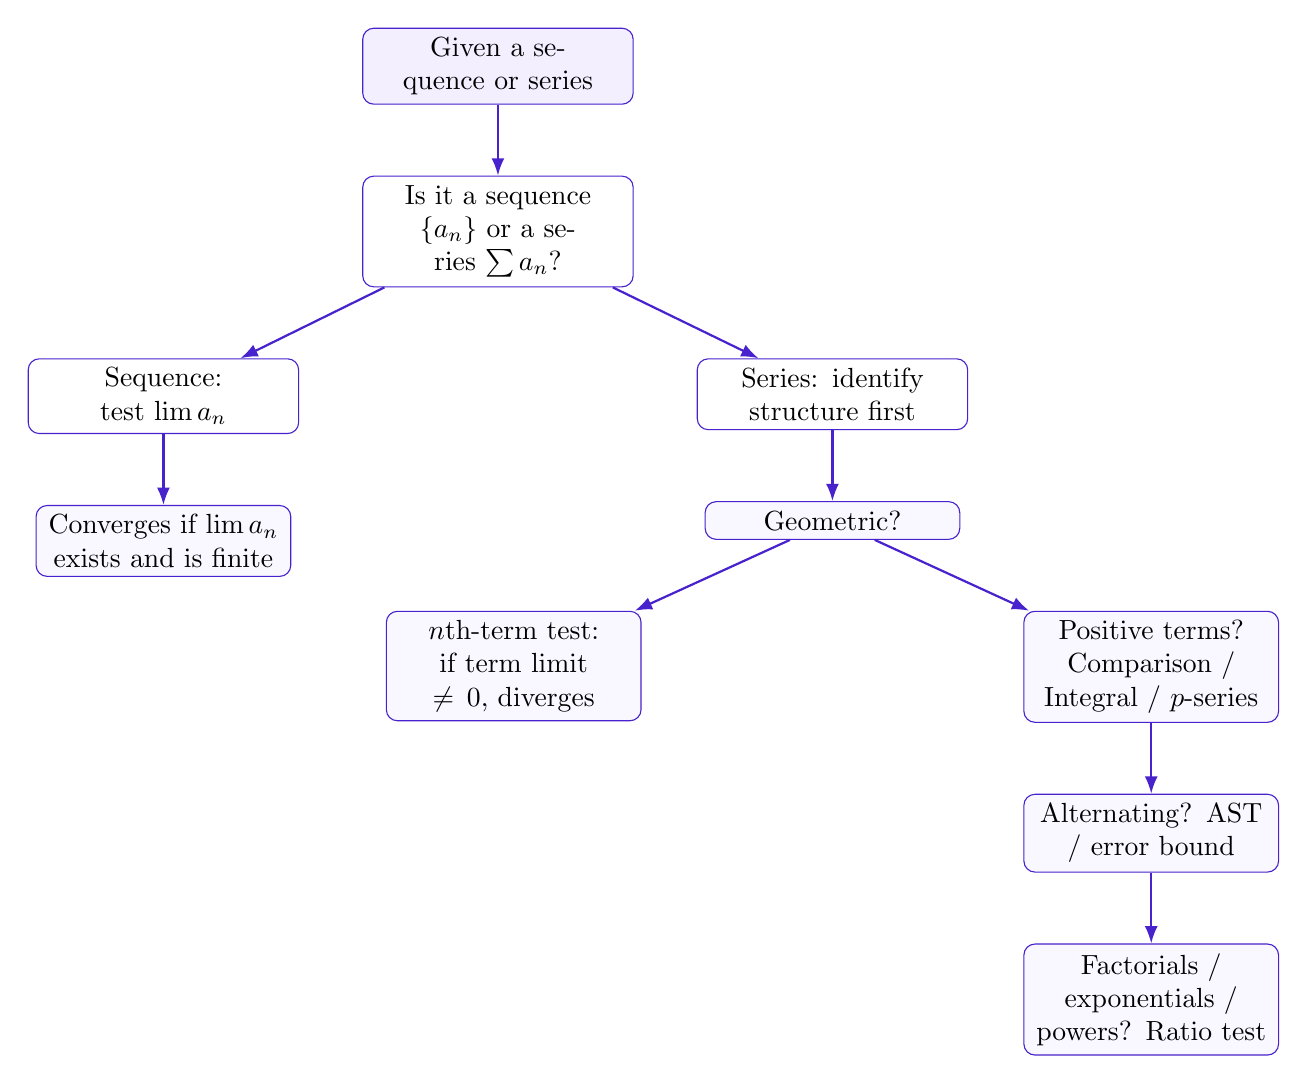
\begin{tikzpicture}[node distance=0.9cm and 0.8cm, scale=1, transform shape]
\node[draw=novelPurpleDark, fill=novelPurpleLight, rounded corners, text width=3.2cm, align=center] (start) {Given a sequence or series};
\node[draw=novelPurpleDark, fill=white, rounded corners, text width=3.2cm, align=center, below=of start] (q1) {Is it a sequence \(\{a_n\}\) or a series \(\sum a_n\)?};
\node[draw=novelPurpleDark, fill=white, rounded corners, text width=3.2cm, align=center, below left=of q1] (seq) {Sequence: test \(\lim a_n\)};
\node[draw=novelPurpleDark, fill=white, rounded corners, text width=3.2cm, align=center, below right=of q1] (series) {Series: identify structure first};

\node[draw=novelPurpleDark, fill=softlav, rounded corners, text width=3.0cm, align=center, below=of seq] (seq2) {Converges if \(\lim a_n\) exists and is finite};

\node[draw=novelPurpleDark, fill=softlav, rounded corners, text width=3.0cm, align=center, below=of series] (s1) {Geometric?};
\node[draw=novelPurpleDark, fill=softlav, rounded corners, text width=3.0cm, align=center, below left=of s1] (s2) {\(n\)th-term test: if term limit \(\neq 0\), diverges};
\node[draw=novelPurpleDark, fill=softlav, rounded corners, text width=3.0cm, align=center, below right=of s1] (s3) {Positive terms? Comparison / Integral / \(p\)-series};
\node[draw=novelPurpleDark, fill=softlav, rounded corners, text width=3.0cm, align=center, below=of s3] (s4) {Alternating? AST / error bound};
\node[draw=novelPurpleDark, fill=softlav, rounded corners, text width=3.0cm, align=center, below=of s4] (s5) {Factorials / exponentials / powers? Ratio test};

\draw[-{Latex[length=2.2mm]}, thick, color=novelPurpleDark] (start)--(q1);
\draw[-{Latex[length=2.2mm]}, thick, color=novelPurpleDark] (q1)--(seq);
\draw[-{Latex[length=2.2mm]}, thick, color=novelPurpleDark] (q1)--(series);
\draw[-{Latex[length=2.2mm]}, thick, color=novelPurpleDark] (seq)--(seq2);
\draw[-{Latex[length=2.2mm]}, thick, color=novelPurpleDark] (series)--(s1);
\draw[-{Latex[length=2.2mm]}, thick, color=novelPurpleDark] (s1)--(s2);
\draw[-{Latex[length=2.2mm]}, thick, color=novelPurpleDark] (s1)--(s3);
\draw[-{Latex[length=2.2mm]}, thick, color=novelPurpleDark] (s3)--(s4);
\draw[-{Latex[length=2.2mm]}, thick, color=novelPurpleDark] (s4)--(s5);
\end{tikzpicture}
\end{center}
\end{summarybox}

\vspace{0.8em}

\begin{summarybox}{Most Common AP BC Question Types}
\renewcommand{\arraystretch}{1.35}
\begin{tabularx}{\textwidth}{@{}p{0.32\textwidth}X@{}}
\toprule
\textbf{Question Type} & \textbf{What You Must Do} \\
\midrule
Sequence convergence & Compute \(\lim_{n\to\infty} a_n\), or explain why it does not exist. \\

Geometric series & Identify \(a\) and \(r\); if \(|r|<1\), find the sum. \\

Divergence test & Check whether \(\lim a_n\neq 0\). If yes, stop immediately: divergent. \\

Comparison test & Compare with a benchmark such as \(\frac1n\), \(\frac1{n^p}\), or a geometric series. \\

Alternating series & Verify positivity, monotone decrease, and limit \(0\). \\

Absolute vs conditional convergence & Test \(\sum |a_n|\) first when appropriate. \\

Alternating error bound & Use the magnitude of the first omitted term. \\

Taylor polynomial approximation & Write the polynomial of requested degree and evaluate it. \\

Error bound question & Use the Lagrange remainder formula and a correct \(M\). \\

Radius / interval of convergence & Use ratio test first, then check endpoints separately. \\

Represent function as power series & Start from a known elementary series and transform it carefully. \\
\bottomrule
\end{tabularx}
\end{summarybox}

\vspace{0.8em}

\begin{summarybox}{Fast Benchmark Memory List}
\begin{itemize}
    \item \(\sum \frac1n\): diverges
    \item \(\sum \frac1{n^p}\): converges iff \(p>1\)
    \item \(\sum ar^n\): converges iff \(|r|<1\)
    \item \(\sum (-1)^{n-1}b_n\): AST works if \(b_n\downarrow 0\)
    \item \(\sum |a_n|\) converges \(\Rightarrow\) \(\sum a_n\) converges
    \item Ratio test is strong for factorials / exponentials / powers to the \(n\)
\end{itemize}
\end{summarybox}


% =========================================================
\newpage
\newpage
\subsection{Homework / Class Exercises}

\begin{homeworkset}{Homework A --- Foundations of Sequences and Series}
\begin{enumerate}
    \item List the first five terms of the sequence \(a_n=\dfrac{2n+1}{n+3}\). Then state whether the sequence appears to converge or diverge.
    \hwspace

    \item Determine whether each sequence converges or diverges:
    \[
    a_n=\frac{3n-1}{2n+5},
    \qquad
    b_n=(-1)^n,
    \qquad
    c_n=\frac{(-1)^n}{n}.
    \]
    \hwspace

    \item Determine whether each series converges or diverges:
    \[
    \sum_{n=1}^{\infty}\frac{1}{3^n},
    \qquad
    \sum_{n=1}^{\infty}1,
    \qquad
    \sum_{n=1}^{\infty}\left(\frac1n-\frac1{n+1}\right).
    \]
    \hwspace

    \item Use the \(n\)th-term test to determine whether
    \[
    \sum_{n=1}^{\infty}\frac{2n}{2n+1}
    \]
    diverges.
\end{enumerate}
\end{homeworkset}
\newpage
\begin{homeworkset}{Homework B --- Convergence Tests}
\begin{enumerate}
\setcounter{enumi}{4}
    \item Apply the Integral Test to
    \[
    \sum_{n=1}^{\infty}\frac{1}{n^2+1}.
    \]
    \hwspace

    \item Classify each as convergent or divergent:
    \[
    \sum_{n=1}^{\infty}\frac{1}{n^{0.8}},
    \qquad
    \sum_{n=1}^{\infty}\frac{1}{n^{3/2}},
    \qquad
    \sum_{n=1}^{\infty}\frac{1}{n}.
    \]
    \hwspace

    \item Use direct comparison to study
    \[
    \sum_{n=1}^{\infty}\frac{1}{n^2+7}.
    \]
    \hwspace

    \item Use limit comparison to study
    \[
    \sum_{n=1}^{\infty}\frac{5n^2+1}{n^4+3}.
    \]
    \hwspace

    \item Determine whether
    \[
    \sum_{n=1}^{\infty}\frac{(-1)^{n-1}}{n^3}
    \]
    is absolutely convergent, conditionally convergent, or divergent.
\end{enumerate}
\end{homeworkset}
\newpage
\begin{homeworkset}{Homework C --- Approximation and Power Series}
\begin{enumerate}
\setcounter{enumi}{9}
    \item How many terms of
    \[
    \sum_{n=1}^{\infty}\frac{(-1)^{n-1}}{n}
    \]
    are needed to guarantee an error less than \(0.005\)?
    \hwspace

    \item Find the fourth-degree Maclaurin polynomial for \(\cos x\).
    \hwspace

    \item Use a third-degree Maclaurin polynomial to approximate \(e^{0.2}\).
    \hwspace

    \item Find the radius and interval of convergence of
    \[
    \sum_{n=1}^{\infty}\frac{x^n}{n\,2^n}.
    \]
    \hwspace

    \item Use a known elementary series to build a power series for
    \[
    \frac{1}{1+x^2}.
    \]
    \hwspace

    \item Find the Maclaurin series for \(\arctan x\) by integrating a geometric-type series.
\end{enumerate}
\end{homeworkset}
\newpage
\begin{homeworkset}{Challenge Problems}
\begin{enumerate}
\setcounter{enumi}{15}
    \item Determine whether
    \[
    \sum_{n=1}^{\infty}\frac{n}{3^n}
    \]
    converges using the Ratio Test.
    \hwspace

    \item Determine whether
    \[
    \sum_{n=1}^{\infty}\frac{n!}{5^n}
    \]
    converges using the Ratio Test.
    \hwspace

    \item Determine whether
    \[
    \sum_{n=1}^{\infty}\frac{(-1)^n}{\sqrt n}
    \]
    is absolutely convergent, conditionally convergent, or divergent.
    \hwspace

    \item Find a power series centered at \(0\) for
    \[
    \frac{x}{(1-x)^2}.
    \]
    \hwspace

    \item Explain clearly why \(\lim a_n=0\) is necessary but not sufficient for
    \[
    \sum a_n
    \]
    to converge.
\end{enumerate}
\end{homeworkset}

% =========================================================
\newpage
\newpage
\subsection{Homework Answer Key}

\begin{theorybox}{Homework A --- Foundations of Sequences and Series}
\begin{enumerate}
    \item
    \[
    a_n=\frac{2n+1}{n+3}
    \]
    First five terms:
    \[
    a_1=\frac34,\quad
    a_2=1,\quad
    a_3=\frac76,\quad
    a_4=\frac95,\quad
    a_5=\frac{11}{8}.
    \]
    The sequence appears to converge, and in fact
    \[
    \lim_{n\to\infty}\frac{2n+1}{n+3}=2.
    \]

    \item
    \[
    a_n=\frac{3n-1}{2n+5}\to \frac32
    \]
    so this sequence converges to \(\frac32\).

    \[
    b_n=(-1)^n
    \]
    alternates between \(1\) and \(-1\), so it diverges.

    \[
    c_n=\frac{(-1)^n}{n}\to 0
    \]
    so it converges to \(0\).

    \item
    \[
    \sum_{n=1}^{\infty}\frac{1}{3^n}
    \]
    is geometric with
    \[
    a=\frac13,\qquad r=\frac13.
    \]
    Since \(|r|<1\), it converges and
    \[
    \sum_{n=1}^{\infty}\frac{1}{3^n}
    =
    \frac{\frac13}{1-\frac13}
    =
    \frac12.
    \]

    \[
    \sum_{n=1}^{\infty}1
    \]
    has partial sums \(S_n=n\), so it diverges.

    \[
    \sum_{n=1}^{\infty}\left(\frac1n-\frac1{n+1}\right)
    \]
    telescopes:
    \[
    S_n=1-\frac1{n+1}\to 1.
    \]
    So it converges to \(1\).

    \item
    \[
    \lim_{n\to\infty}\frac{2n}{2n+1}=1\neq 0.
    \]
    Therefore,
    \[
    \sum_{n=1}^{\infty}\frac{2n}{2n+1}
    \]
    diverges by the \(n\)th-term test.
\end{enumerate}
\end{theorybox}

\begin{theorybox}{Homework B --- Convergence Tests}
\begin{enumerate}
\setcounter{enumi}{4}
    \item
    Let
    \[
    f(x)=\frac{1}{x^2+1}.
    \]
    Since \(f\) is continuous, positive, and decreasing for \(x\ge 1\), the Integral Test applies.
    \[
    \int_1^{\infty}\frac{1}{x^2+1}\,dx
    =
    \lim_{b\to\infty}[\arctan x]_1^b
    =
    \frac{\pi}{2}-\frac{\pi}{4}
    =
    \frac{\pi}{4}.
    \]
    Because the improper integral converges, the series
    \[
    \sum_{n=1}^{\infty}\frac{1}{n^2+1}
    \]
    converges.

    \item
    \[
    \sum_{n=1}^{\infty}\frac{1}{n^{0.8}}
    \]
    is a \(p\)-series with \(p=0.8<1\), so it diverges.

    \[
    \sum_{n=1}^{\infty}\frac{1}{n^{3/2}}
    \]
    is a \(p\)-series with \(p=\frac32>1\), so it converges.

    \[
    \sum_{n=1}^{\infty}\frac{1}{n}
    \]
    is the harmonic series, so it diverges.

    \item
    Since
    \[
    0<\frac{1}{n^2+7}<\frac{1}{n^2},
    \]
    and
    \[
    \sum_{n=1}^{\infty}\frac{1}{n^2}
    \]
    converges, the series
    \[
    \sum_{n=1}^{\infty}\frac{1}{n^2+7}
    \]
    converges by direct comparison.

    \item
    Compare with
    \[
    b_n=\frac{1}{n^2}.
    \]
    Then
    \[
    \lim_{n\to\infty}
    \frac{\frac{5n^2+1}{n^4+3}}{\frac{1}{n^2}}
    =
    \lim_{n\to\infty}\frac{n^2(5n^2+1)}{n^4+3}
    =
    5.
    \]
    Since \(0<5<\infty\), the given series has the same behavior as
    \[
    \sum_{n=1}^{\infty}\frac{1}{n^2},
    \]
    so it converges.

    \item
    Consider
    \[
    \sum_{n=1}^{\infty}\left|\frac{(-1)^{n-1}}{n^3}\right|
    =
    \sum_{n=1}^{\infty}\frac{1}{n^3}.
    \]
    This is a \(p\)-series with \(p=3>1\), so it converges.
    Therefore the original series is \textbf{absolutely convergent}.
\end{enumerate}
\end{theorybox}

\begin{theorybox}{Homework C --- Approximation and Power Series}
\begin{enumerate}
\setcounter{enumi}{9}
    \item
    For
    \[
    \sum_{n=1}^{\infty}\frac{(-1)^{n-1}}{n},
    \]
    the alternating-series error bound says
    \[
    |S-S_N|\le \frac{1}{N+1}.
    \]
    We want
    \[
    \frac{1}{N+1}<0.005.
    \]
    Since \(0.005=\frac{1}{200}\), we need
    \[
    N+1>200.
    \]
    So \(N=200\) terms are sufficient.

    \item
    The fourth-degree Maclaurin polynomial for \(\cos x\) is
    \[
    P_4(x)=1-\frac{x^2}{2!}+\frac{x^4}{4!}.
    \]

    \item
    The third-degree Maclaurin polynomial for \(e^x\) is
    \[
    P_3(x)=1+x+\frac{x^2}{2!}+\frac{x^3}{3!}.
    \]
    So
    \[
    e^{0.2}\approx P_3(0.2)
    =1+0.2+\frac{0.2^2}{2}+\frac{0.2^3}{6}.
    \]
    Compute:
    \[
    1+0.2+0.02+\frac{0.008}{6}
    =1.22+0.001333\ldots
    =1.221333\ldots
    \]

    \item
    Consider
    \[
    \sum_{n=1}^{\infty}\frac{x^n}{n\,2^n}.
    \]
    Using the Ratio Test:
    \[
    \left|\frac{a_{n+1}}{a_n}\right|
    =
    \left|
    \frac{x^{n+1}}{(n+1)2^{n+1}}
    \cdot
    \frac{n2^n}{x^n}
    \right|
    =
    \left|\frac{x}{2}\cdot\frac{n}{n+1}\right|
    \to \left|\frac{x}{2}\right|.
    \]
    So the series converges when
    \[
    \left|\frac{x}{2}\right|<1
    \quad\Longrightarrow\quad
    |x|<2.
    \]
    Thus \(R=2\).

    Check endpoints:
    \begin{itemize}
        \item At \(x=2\):
        \[
        \sum_{n=1}^{\infty}\frac{2^n}{n2^n}
        =
        \sum_{n=1}^{\infty}\frac1n
        \]
        diverges.
        \item At \(x=-2\):
        \[
        \sum_{n=1}^{\infty}\frac{(-2)^n}{n2^n}
        =
        \sum_{n=1}^{\infty}\frac{(-1)^n}{n}
        \]
        converges.
    \end{itemize}
    Therefore the interval of convergence is
    \[
    [-2,2).
    \]

    \item
    Consider
    \[
    \sum_{n=1}^{\infty}\frac{(x-1)^n}{n\,4^n}.
    \]
    Ratio Test:
    \[
    \left|\frac{a_{n+1}}{a_n}\right|
    =
    \left|\frac{x-1}{4}\cdot\frac{n}{n+1}\right|
    \to \left|\frac{x-1}{4}\right|.
    \]
    So convergence occurs when
    \[
    |x-1|<4.
    \]
    Hence \(R=4\), with candidate interval
    \[
    -3<x<5.
    \]

    Check endpoints:
    \begin{itemize}
        \item At \(x=5\):
        \[
        \sum_{n=1}^{\infty}\frac{4^n}{n4^n}
        =
        \sum_{n=1}^{\infty}\frac1n
        \]
        diverges.
        \item At \(x=-3\):
        \[
        \sum_{n=1}^{\infty}\frac{(-4)^n}{n4^n}
        =
        \sum_{n=1}^{\infty}\frac{(-1)^n}{n}
        \]
        converges.
    \end{itemize}
    Therefore the interval of convergence is
    \[
    [-3,5).
    \]

    \item
    Start from the geometric series
    \[
    \frac{1}{1-u}=\sum_{n=0}^{\infty}u^n,\qquad |u|<1.
    \]
    Let \(u=-x^2\). Then
    \[
    \frac{1}{1+x^2}
    =
    \frac{1}{1-(-x^2)}
    =
    \sum_{n=0}^{\infty}(-x^2)^n
    =
    \sum_{n=0}^{\infty}(-1)^n x^{2n},
    \qquad |x|<1.
    \]

    \item
    Start from
    \[
    \frac{1}{1+x}
    =
    \sum_{n=0}^{\infty}(-1)^n x^n,
    \qquad |x|<1.
    \]
    Integrate term by term from \(0\) to \(x\):
    \[
    \ln(1+x)
    =
    \sum_{n=0}^{\infty}(-1)^n\frac{x^{n+1}}{n+1}
    =
    \sum_{n=1}^{\infty}(-1)^{n-1}\frac{x^n}{n}.
    \]
    Since
    \[
    \frac{d}{dx}(\arctan x)=\frac{1}{1+x^2},
    \]
    integrate
    \[
    \frac{1}{1+x^2}
    =
    \sum_{n=0}^{\infty}(-1)^n x^{2n}
    \]
    term by term:
    \[
    \arctan x
    =
    \sum_{n=0}^{\infty}(-1)^n\frac{x^{2n+1}}{2n+1}.
    \]
\end{enumerate}
\end{theorybox}

\begin{theorybox}{Challenge Problems}
\begin{enumerate}
\setcounter{enumi}{15}
    \item
    Let
    \[
    a_n=\frac{n}{3^n}.
    \]
    Then
    \[
    \left|\frac{a_{n+1}}{a_n}\right|
    =
    \frac{(n+1)/3^{n+1}}{n/3^n}
    =
    \frac{n+1}{3n}\to \frac13<1.
    \]
    Therefore the series converges absolutely.

    \item
    Let
    \[
    a_n=\frac{n!}{5^n}.
    \]
    Then
    \[
    \left|\frac{a_{n+1}}{a_n}\right|
    =
    \frac{(n+1)!/5^{n+1}}{n!/5^n}
    =
    \frac{n+1}{5}.
    \]
    As \(n\to\infty\),
    \[
    \frac{n+1}{5}\to\infty>1.
    \]
    Therefore the series diverges.

    \item
    Consider
    \[
    \sum_{n=1}^{\infty}\frac{(-1)^n}{\sqrt n}.
    \]
    The absolute value series is
    \[
    \sum_{n=1}^{\infty}\frac{1}{\sqrt n},
    \]
    which is a \(p\)-series with \(p=\frac12<1\), so it diverges.

    But the alternating series itself converges by the Alternating Series Test because
    \[
    \frac{1}{\sqrt n}\downarrow 0.
    \]
    Therefore the series is \textbf{conditionally convergent}.

    \item
    Start from
    \[
    \frac{1}{1-x}=\sum_{n=0}^{\infty}x^n,\qquad |x|<1.
    \]
    Differentiate:
    \[
    \frac{1}{(1-x)^2}
    =
    \sum_{n=1}^{\infty}n x^{n-1}.
    \]
    Multiply by \(x\):
    \[
    \frac{x}{(1-x)^2}
    =
    \sum_{n=1}^{\infty}n x^n,
    \qquad |x|<1.
    \]

    \item
    The condition
    \[
    \lim_{n\to\infty}a_n=0
    \]
    is necessary because every convergent series must have terms approaching \(0\).

    However, it is not sufficient. A standard counterexample is the harmonic series:
    \[
    \sum_{n=1}^{\infty}\frac1n.
    \]
    Here
    \[
    \lim_{n\to\infty}\frac1n=0,
    \]
    but the series still diverges. So terms going to \(0\) is only a first checkpoint, not a proof of convergence.
\end{enumerate}
\end{theorybox}


% =========================================================
\newpage
\subsection{Unit 10 Final Teaching Checklist}

\begin{theorybox}{Before Leaving Unit 10, Students Should Comfortably Handle}
\begin{itemize}
    \item distinguishing sequences from series
    \item interpreting convergence through partial sums
    \item recognizing geometric-series structure immediately
    \item knowing that the \(n\)th-term test proves divergence, not convergence
    \item selecting among Integral, Comparison, Alternating, and Ratio Tests
    \item classifying absolute versus conditional convergence
    \item estimating alternating-series approximation error
    \item building Taylor polynomials and using remainder bounds
    \item finding radius and interval of convergence
    \item generating new series from known elementary ones by substitution, differentiation, and integration
\end{itemize}
\end{theorybox}

\vfill
\begin{center}
{\Large\color{novelPurpleDark}\textbf{End of Unit 10}}\\[0.35em]
{\large Infinite Sequences and Series}
\end{center}

\end{document}